%! TEX program = lualatex

% TODO: remove onecolumn and draftcls formatting
\documentclass[journal,twoside,web, twocolumn,draftcls]{ieeecolor}

\usepackage{generic}
%/========== Preamble ==========/%
% Packages required by ieeecolor
\usepackage{amsmath}
\usepackage{amsfonts}
\usepackage{amssymb}
\usepackage{algorithmic}
\usepackage{graphicx}
\usepackage{subcaption}
\usepackage{textcomp}
\usepackage{cite}

%---------- More packages ----------%
% NOTE: cannot use amsthm for some reason
\usepackage{mathtools}
\usepackage{bm}
\usepackage{booktabs}

%---------- Bibliography Style ----------%
\bibliographystyle{IEEEtran}

%---------- Header ----------% 
\newcommand*{\Title}{From gymnastics to virtual nonholonomic constraints: energy
injection, dissipation, and regulation for the acrobot}
\markboth{\journalname, VOL. XX, NO. XX, XXXX 2021}
{Moran-MacDonald \MakeLowercase{\textit{et al.}}: \Title}

%---------- Theorems ----------%
\newtheorem{thm}{Theorem}% Uncomment: reset numbering at each chapter
\newtheorem{prop}{Proposition} % Propositions don't depend on Theorem number
\newtheorem{lemma}{Lemma} % Same with lemmas
\newtheorem{defn}{Definition} % Definitions do not depend on theorem number
\newtheorem{assm}{Assumption} % Assumptions do not reset 

%---------- Special Commands ----------%
\DeclarePairedDelimiter{\norm}{\lVert}{\rVert}
\DeclarePairedDelimiter{\abs}{\lvert}{\rvert}
\DeclareMathOperator{\Rank}{rank}
\DeclareMathOperator{\Sign}{sgn}
\DeclareMathOperator{\Diag}{diag}
\newcommand*{\rank}[1]{\Rank\left(#1\right)}
\newcommand*{\sign}[1]{\Sign\left(#1\right)}
\newcommand*{\diag}[1]{\Diag\left(#1\right)}

\newcommand*{\tpose}{^\mathsf{T}} 
\newcommand*{\inv}{^\mathsf{-1}}
\newcommand*{\Rt}[1]{[\R]_{#1}}
\newcommand*{\R}{\mathbb{R}}
\newcommand*{\n}{\mathbf{n}}
\newcommand*{\N}{\mathbb{N}}
\newcommand*{\Sone}{\mathbb{S}^1}
\newcommand*{\SxR}{\Sone \times \R}
\newcommand*{\Minv}{M^\mathsf{-1}}
\newcommand*{\Id}[1]{I_{#1}}
\newcommand*{\Zmat}[1]{\bm{0}_{#1}}
\newcommand*{\diff}[2]{\frac{d #1}{d #2}}
\newcommand*{\ddiff}[3]{\frac{d^2 #1}{d #2 d #3}}
\newcommand*{\pdiff}[2]{\frac{\partial #1}{\partial #2}}

\newcommand*{\simpleB}{\begin{bmatrix}\Zmat{(n-k)\times k}\\ \Id{k}\end{bmatrix}}
\newcommand*{\pdmat}{(\Id{n} \otimes p\tpose)\nabla_q\Minv(q)p}
\newcommand*{\pudmat}{(\Id{n-k} \otimes p\tpose)\nabla_{q_u}\Minv(q)p}

\newcommand*{\etal}{\MakeLowercase{\textit{et al.~}}}
%/========== /Preamble ==========/%

%/========== Main Document ==========/%
\begin{document}
\title{\Title}
\author{Adan Moran-MacDonald, \IEEEmembership{Member, IEEE}, Manfredi Maggiore,
\IEEEmembership{Member, IEEE}*, and Xingbo Wang
\thanks{Manuscript submitted for review on \today.}
\thanks{A. Moran-MacDonald (e-mail: adan.moran@mail.utoronto.ca) and
M. Maggiore (e-mail: maggiore@control.utoronto.ca) are with the Department of
Electrical and Computer Engineering, University of Toronto, ON, Canada.}
\thanks{X. Wang is with ??? (e-mail: ???).}
} %/author

\maketitle

%/========== Abstract ==========/%
\begin{abstract}
    In this article we study virtual nonholonomic constraints, which are
    relations between the generalized coordinates and generalized momenta of a
    mechanical system that can be enforced via feedback control.
    We design a constraint which emulates gymnastics giant motion in an
    acrobot, and rigorously prove that this constraint will inject or dissipate
    energy.
    This constraint is tested in simulation and on a real-world acrobot,
    demonstrating highly effective energy regulation properties and robustness
    to a variety of disturbances.
\end{abstract}

\begin{IEEEkeywords}
    energy regulation, virtual nonholonomic constraints, acrobot, gymnastics.
\end{IEEEkeywords}

%/========== Introduction ==========/%
\section{Introduction}\label{sec:introduction}

In gymnastics terminology, a ``giant" is the motion a gymnast performs to
achieve full rotations around a horizontal bar \cite{usagym_giant}. 
A gymnast will begin by hanging at rest, then swing their legs
appropriately to gain energy over time.
The authors of \cite{pendulum_length_giant_gymnastics} modelled the gymnast as a
variable length pendulum, and studied how the pendulum's length changes as a
function of the gymnast's limb angle.
Labeling the pendulum length by \(r\) and the gymnast's body orientation
by \(\theta\), they observed experimentally that the value \(\dot{r}/r\) has
the biggest impact on the magnitude of energy injection. 
After testing several gymnasts under a variety of experimental conditions, 
they discovered that the peak value of \(\dot{r}/r\) occured at the same fixed
value of \(\dot{\theta}/\theta\) for all gymnasts.
In other words, gymnasts appear to move their legs as a function of their body
angle and velocity when performing giants; 
doing so allows them to gain energy and rotate around the bar.

While the simplest model of a gymnast is the variable-length pendulum, a
more realistic model is the two-link acrobot (Figure \ref{fig:acrobot}).
Here, the top link represents the torso while the bottom link represents
the legs. 
The acrobot is actuated exclusively at the center joint (the hip).
Controlling the acrobot is a nontrivial task because it is not feedback
linearizable \cite{nonlinear_controllers_nonintegrable_acrobot}. 
To solve the swingup problem, one might begin by designing a leg controller
which provably injects energy into the acrobot, so that the resulting motion
mimics that of a human performing a giant.

\begin{figure}
    \centering
    \begin{subfigure}[t]{0.40\linewidth}
        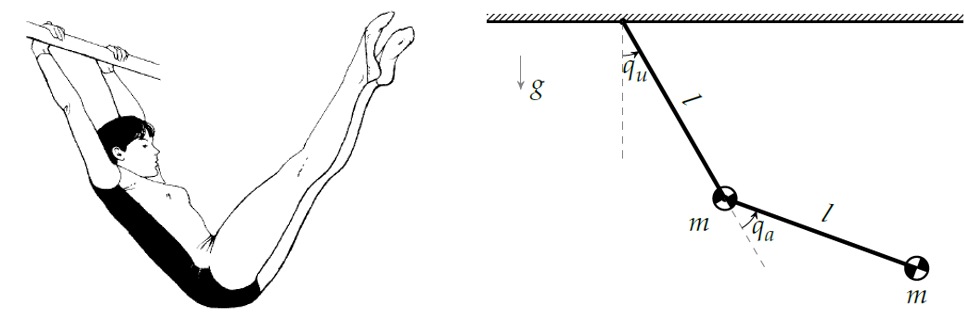
\includegraphics[width=\linewidth]{acrobot_gymnast.png}
    \end{subfigure}
    \hfill
    \begin{subfigure}[t]{0.48\linewidth}
        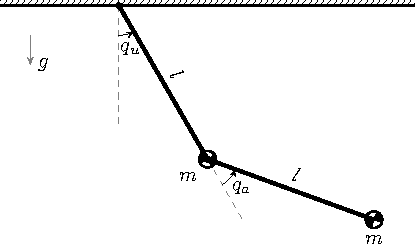
\includegraphics[width=\linewidth]{simple_acrobot_model.pdf}
    \end{subfigure}
    \caption{A simplified two-link acrobot as a model for a gymnast.
    Image modified from \cite{xingbo_thesis}.}
    \label{fig:acrobot}
\end{figure}

Previous attempts at acrobot giant generation have involved
trajectory tracking, partial feedback linearization, or other energy-based
methods
( see
\cite{energy_pumping_robotic_swinging,swingup_giant_acrobot,dynamical_servo_acrobot_vc,control_giant_two_link_gymnastic_robot}
).
While all these approaches succeed at making the acrobot rotate around the
bar, none of them use the results of \cite{pendulum_length_giant_gymnastics}.
That is, none of these leg controllers track a function of the acrobot's body
angle and velocity.
In 2016, Wang designed a controller \cite{xingbo_thesis} which tracked the
body angle and an \textit{estimate} of the velocity, but not the velocity itself.
His approach was a preliminary version of a recent technique know as the method
of virtual nonholonomic constraints \cite{hybrid_zero_dynamics_bipedal_nhvcs}.

Virtual nonholonomic constraints (VNHCs) have been used for human-robot interaction
\cite{vnhc_human_robot_cooperation,psd_based_vnhc_redundant_manipulator,haptic_vnhc},
error-reduction on time-delayed systems \cite{vnhc_time_delay_teleop},
and they have shown marked improvements to the field of bipedal locomotion 
\cite{nhvc_dynamic_walking,
hybrid_zero_dynamics_bipedal_nhvcs,output_nhvc_bipedal_control}.
Indeed, they produce more robust walking motion in biped robots than
other virtual constraints which do not depend on velocity
\cite{nhvc_incline_walking}.
In particular, VNHCs may be capable of injecting and
dissipating energy from a system in a robust manner, all while producing
realistic biological motion. 

In this article, we design a virtual nonholonomic constraint which provably
injects energy into the acrobot through human-like giant motion.
In particular, any acrobot constrained by this VNHC is guaranteed to perform
rotations around the bar.
Under suitable conditions on the acrobot's physical parameters, this VNHC
also enables the acrobot to rotate around the bar at a desired speed.
We will provide simulations to show how one can use VNHCs to regulate energy,
along with experimental results which demonstrate the robustness of this
behaviour to model uncertainty, sensor noise, and a variety of external
disturbances. 

%%
\textbf{Notation}:
%%
We use the following notation and terminology in this article.
The \(n \times n\) identity matrix is denoted \(\Id{n}\), and the \(n \times m\)
matrix of zeros is denoted \(\Zmat{n\times m}\).
A matrix \(A \in \R^{n \times m}\) is \textit{right semi-orthogonal} if
\(A A\tpose = \Id{n}\) and is \textit{left semi-orthogonal} if 
\(A\tpose A = \Id{m}\).
For \(A \in \R^{n\times m}\) and \(B \in \R^{p \times m}\),
we define \([A;B] \in \R^{(n+p)\times m}\) as the matrix obtained by stacking \(A\)
on top of \(B\). 
Given \(\sigma_1,\ldots,\sigma_n \in \R\), we define 
\(\diag{\sigma_1,\ldots,\sigma_n} \in \R^{n \times n}\) as the diagonal matrix
whose value at row \(i\), column \(i\) is \(\sigma_i\).
For \(T > 0\), the set of real numbers modulo \(T\) is denoted \(\Rt{T}\), with
\(\Rt{\infty} := \R\).
The gradient of a matrix-valued function 
\(A : \R^m \rightarrow \R^{n\times n}\) is the block matrix of stacked partial
derivatives, 
\(\nabla_xA := [\partial A/\partial x_1; \cdots; \partial A/\partial x_m] \in
\R^{nm \times n}\).
%\(\nabla_xA := [\pdiff{A}{x_1};\ldots;\pdiff{A}{x_m}] \in \R^{nm \times n}\).
Given two matrices \(A \in \R^{n \times m}\) and \(B \in \R^{r \times s}\), the
Kronecker product (see \cite{kronprod}) is the matrix  
\(A \otimes B \in \R^{nr \times ms}\)  defined as
\begin{equation}\label{eqn:kronprod}
    A \otimes B = \begin{bmatrix}
        A_{1,1}B & \cdots & A_{1,m} B \\
        \vdots & \ddots & \vdots \\
        A_{n,1} B & \cdots & A_{n,m} B
    \end{bmatrix} 
    .
\end{equation}
The Poisson bracket \cite{landau_mechanics} between the functions
\(f(q,p)\) and \(g(q,p)\) is
\begin{equation}\label{eqn:poisson-bracket}
    [f,g] := \sum \limits_{i=1}^n \pdiff{f}{p_i}\pdiff{g}{q_i} - 
        \pdiff{f}{q_i}\pdiff{g}{p_i}
    .
\end{equation}
The Kronecker delta \(\delta_i^j\) is \(1\) if \(i = j\) and \(0\)
otherwise.
Finally, we say a function \(R(I)\) is \(O(I^2)\)
if \(\lim_{I \to 0} R(I)/I = 0\).

%/========== Problem Formulation ==========/%
\section{Problem Formulation}\label{sec:problem-formulation}
We will use the simplified acrobot model in Figure
\ref{fig:acrobot}, where we assume the torso and leg rods are of
equal length \(l\) with equal point masses \(m\) at the tips.
The acrobot's configuration is described in generalized coordinates
\((q_u,q_a)\) on the configuration manifold 
\(\mathcal{Q} = \Sone \times \Sone\), where \(q_u\) is unactuated and 
\(q_a\) is actuated.
A real gymnast cannot swing their legs in full circles, though they
are usually flexible enough to raise them parallel to the floor;
hence, we assume the leg angle \(q_a\) lies in \([-Q_a, Q_a]\) for some
\(Q_a \in [\frac{\pi}{2}, \pi[\). 
We also ignore any dissipative forces.

The acrobot has inertia matrix 
\(M\), potential function \(V\) (with respect to
the horizontal bar), and input matrix \(B\) given as follows:
\begin{align}\label{eqn:acrobot-inertia}
    M(q) &= \begin{bmatrix}
        ml^2\left(3+2\cos(q_a)\right) & 
        ml^2\left(1+\cos(q_a)\right) \\
        ml^2\left(1+\cos(q_a)\right) &
        ml^2
    \end{bmatrix} 
    , \\
    \label{eqn:acrobot-potential}
    V(q) &= -mgl\left(2\cos(q_u)+\cos(q_u+q_a)\right)
    , \\
    \label{eqn:acrobot-B}
    B &= [0;1]
    .
\end{align}
For reasons that will become clear in later sections of this article, we will
use Hamiltonian mechanics to derive the dynamics of the acrobot. 
For this we require the conjugate of momenta, \(p = (p_u,p_a) = M(q)\dot{q}\).
The dynamics of the acrobot in \((q,p)\) coordinates are given in
\eqref{eqn:acrobot-hamiltonian}.
For shorthand, we write \(c_u := \cos(q_u)\), \(c_a := \cos(q_a)\), and 
\(c_{ua} := \cos(q_u + q_a)\); likewise, \(s_u := \sin(q_u)\), 
\(s_a := \sin(q_a)\), and \(s_{ua} := \sin(q_u + q_a)\).
\begin{align}\label{eqn:acrobot-hamiltonian}
    \mathcal{H}(q,p) &= \frac{1}{2}p\tpose \Minv(q) p -
    mgl\left(2 c_u + c_{ua}\right)
    , \\
     &\begin{cases}
        \dot{q} = \Minv(q) p 
        ,\\
        \dot{p}_u = -mgl\left(2s_u + s_{ua}\right) 
        ,\\
        \dot{p}_a =-\frac{1}{2}p\tpose \nabla_{q_a}\Minv(q) p
        - mgl s_{ua} + \tau.
    \end{cases} \nonumber
\end{align}
The control input is a force \(\tau \in \R\) affecting only the dynamics of
\(p_a\), representing a torque acting on the hip joint.
Let us now define what it means for a mechanical system to gain or lose energy.

\begin{defn}\label{defn:energy-gain}
    Let \(\mathcal{Q}\) be an
    \(n\)-dimensional smooth manifold. 
    Let \(f : \mathcal{Q} \rightarrow T\mathcal{Q}\) be a smooth vector
    field and let \(D \subset \mathcal{Q}\) be open.
    The system described by \(\dot{x} = f(x)\) 
    \textit{gains energy on \(D\)} if, 
    for all compact sets \(K \subset D\) and for almost every initial
    condition \(x(0) \in K\), there exists \(T > 0\) such
    that \(x(t) \notin K\) for all \(t > T\).
    The system \textit{loses energy on \(D\)} if it gains energy in
    negative-time.
\end{defn}

The definition above applies to vector fields that are a not necessarily
Hamiltonian, and therefore might not have an associated notion of ``energy". 
The terms ``gain energy" and ``lose energy" are to be interpreted loosely in
this context.
Our goal is to design a smooth function \(f : \Sone \times \R\) such that the
relation \(q_a = f(q_u,p_u)\) for system \eqref{eqn:acrobot-hamiltonian}
can be enforced asymptotically via feedback control (in Section \ref{sec:vnhc}
we call this a regular virtual nonholonomic constraint).  
We will further require that the dynamics of the acrobot, when the relation
holds, gain or lose energy on some set \(D\) in the sense of Definition
\ref{defn:energy-gain}. 
Note that any system satisfying Definition \ref{defn:energy-gain}
can have unstable equilibria on \(D\), but not limit cycles nor closed orbits.

%/========== VNHC ==========/%
\section{Theory of VNHCs}\label{sec:vnhc}
Before embarking on our design problem, we must summarize the relevant
theory of virtual nonholonomic constraints for a class of mechanical systems we
call ``simply actuated hamiltonian systems". 
The results we provide in Section \ref{sec:vnhc-vnhc} are not novel:
they are a special case of the results in
\cite{hybrid_zero_dynamics_bipedal_nhvcs}.

\subsection{Simply Actuated Hamiltonian Systems} \label{sec:vnhc-sah}
Take a mechanical system modelled with generalized coordinates 
\(q = (q_1, \ldots, q_n)\) on a configuration manifold
\(\mathcal{Q} = \Rt{T_1} \times \cdots \times \Rt{T_n}\), where
\(T_i = 2\pi\) if \(q_i\) is an angle and \(T_i = \infty\) if \(q_i\) is a
displacement. The corresponding generalized velocities are 
\(\dot{q} = (\dot{q}_1,\ldots,\dot{q}_n) \in \R^n\).

Suppose this system has Lagrangian
\(\mathcal{L}(q,\dot{q}) = 1/2~\dot{q}^T D(q) \dot{q} - P(q)\),
where the potential energy 
\(P : \mathcal{Q} \rightarrow \mathbb{R}\) 
is smooth, and the inertia matrix 
\(D : \mathcal{Q} \rightarrow \mathbb{R}^{n \times n}\)
is smooth and positive definite for all \(q \in \mathcal{Q}\).
The \textit{conjugate of momentum} to \(q\) is the vector
\(p := \partial\mathcal{L}/\partial\dot{q} = D(q) \dot{q} \in \R^n\).
As per \cite{landau_mechanics}, 
the \textit{Hamiltonian} of the system in \((q,p)\) coordinates
is
\begin{equation}\label{eqn:hamiltonian}
    \mathcal{H}(q,p) = \frac{1}{2} p\tpose D\inv(q) p + P(q)
    ,
\end{equation}
with dynamics
\begin{equation}\label{eqn:hamiltonian-eom-general}
    \begin{cases}
        \dot{q} = \nabla_p\mathcal{H} 
        , \\
        \dot{p} = -\nabla_q\mathcal{H} + B(q) \tau
        ,
    \end{cases}
\end{equation}
where \(\tau \in \R^k\) is a vector of generalized input forces and the input
matrix \(B : \mathcal{Q} \rightarrow \R^{n \times k}\) is full rank for all 
\(q \in \mathcal{Q}\).
If \(k < n\), we say the system is \textit{underactuated} with degree of
underactuation \((n-k)\).

Using the matrix Kronecker product, it is easy to show that
\eqref{eqn:hamiltonian-eom-general} expands to
\begin{equation*}\label{eqn:hamiltonian-full-dynamics}
     \begin{cases}
        \dot{q} = D\inv(q)p 
        , \\
        \dot{p} = -\frac{1}{2} (\Id{n} \otimes p\tpose) \nabla_q D\inv(q) p
        - \nabla_q P(q) + B(q) \tau
        . \\
    \end{cases}
\end{equation*}
%\begin{align*}
%    \dot{q} &= D\inv(q)p 
%    ,\\
%    \dot{p} &= -\frac{1}{2} (\Id{n} \otimes p\tpose) \nabla_q D\inv(q) p
%        - \nabla_q P(q) + B(q) \tau
%    .
%\end{align*}

Because \(\tau\) is transformed by \(B(q)\), it is not obvious how any
particular input force \(\tau_i\) affects the system.
As a first step in addressing this problem, we make the following assumptions.

\begin{assm}\label{assm:B-const}
    The input matrix \(B(q) \equiv B \in \R^{n\times k}\) is constant
    and has full rank \(k < n\).
\end{assm}

%\begin{assm}\label{assm:B-perp}
%    There exists a right semi-orthogonal matrix 
%    \(B^\perp \in \R^{(n-k)\times n}\)
%    which is a left-annihilator for \(B\). 
%\end{assm}
%
%Note that Assumption \ref{assm:B-perp} requires the rows of \(B^\perp\) be unit vectors
%that are mutually orthogonal. 
%When \(k = (n-1)\), Assumption \ref{assm:B-perp} can be removed because it is
%automatically implied by Assumption \ref{assm:B-const}.
%
When \(\mathcal{Q} = \R^n\), the above assumption allows us to define a
canonical coordinate transformation of \eqref{eqn:hamiltonian} 
which decouples the input forces.
To define this transformation we will make use of the following lemma.

\begin{lemma}\label{lemma:B-orthogonal}
    Suppose Assumption \ref{assm:B-const} holds. Then
    there exists a nonsingular matrix \(\hat{T} \in \R^{k \times k}\) 
    so that the regular feedback transformation 
    \[
        \tau = \hat{T} \hat{\tau}
    \] 
    has a new input matrix \(\hat{B}\) for \(\hat{\tau}\) which is left
    semi-orthogonal.  
\end{lemma}
\begin{proof}
    Since \(B\) is constant and full rank, it has a singular value decomposition 
    \(B = U\tpose \Sigma V\) where 
    \(\Sigma = [\diag{\sigma_1,\ldots,\sigma_k}; \Zmat{(n-k)\times k}]\),
    \(\sigma_i > 0\), and \(U \in R^{n \times n}\),
    \(V \in \R^{k \times k}\) are unitary matrices \cite{calculating_svd}.
    Defining \(T = \diag{1/\sigma_1,\ldots,1/\sigma_k}\) and assigning the
    regular feedback transformation \(\tau = V T \hat{\tau}\) yields a new input
    matrix \(\hat{B} = B V T\) for \(\hat{\tau}\) such that
    \(\hat{B}\tpose \hat{B} = T\tpose \Sigma\tpose \Sigma T = \Id{k}\).
\end{proof}

In light of Lemma \ref{lemma:B-orthogonal} there is no loss of generality in
assuming that the input matrix is left semi-orthogonal, which means that
\(B\tpose\) is right semi-orthogonal.
Now, let \(\mathbf{B} := [B^\perp; B\tpose]\) where 
\(B^\perp \in \R^{(n-k)\times k}\) is a left annihilator of \(B\), i.e.,
\(B^\perp B = \Zmat{(n-k) \times k}\).
Since \(B\) is constant, such a \(B^\perp\) exists and
\(\mathbf{B}\) is invertible.

The following theorem requires that \(\mathcal{Q} = \R^n\) so that the
transformation \(\tilde{q} = \mathbf{B}q\) is well defined.

\begin{thm}\label{thm:simply-actuated}
    Take the Hamiltonian system \eqref{eqn:hamiltonian} with configuration
    manifold \(\mathcal{Q} = \R^n\) and suppose
    Assumption \ref{assm:B-const} holds.
    The coordinate transformation
    \(\left(\tilde{q} = (\mathbf{B}\tpose)\inv q, \tilde{p} = \mathbf{B}p\right)\)
    is a canonical transformation and the resulting dynamics are given by 
    \begin{gather}\label{eqn:simple-hamiltonian}
        \mathcal{H}(\tilde{q},\tilde{p}) = 
        \frac{1}{2} \tilde{p}\tpose \Minv(\tilde{q}) \tilde{p} + V(\tilde{q})
        , \\
       \begin{cases}
           \dot{\tilde{q}} = \Minv(\tilde{q})\tilde{p}
           , \\
           \dot{\tilde{p}} = -\frac{1}{2} (\Id{n} \otimes \tilde{p}\tpose)
           \nabla_{\tilde{q}} \Minv(\tilde{q}) \tilde{p} \\
           \phantom{---} - \nabla_{\tilde{q}} V(\tilde{q}) + \simpleB \tau
            ,
        \end{cases} \nonumber
    \end{gather}
    where 
    \(\Minv(\tilde{q}) := 
    (\mathbf{B}\tpose)\inv D^{-1}(\mathbf{B}\tpose \tilde{q})\mathbf{B}\inv\)
    and
    \(V(\tilde{q}) := P(\mathbf{B}\tpose \tilde{q})\).
\end{thm}
\begin{proof}
    Since \(\mathbf{B}\) is constant, this transformation satisfies
    \(\partial\tilde{q}_i/\partial p_j = \partial\tilde{p}_i/\partial q_j = 0\) for all 
    \(i,j \in \{1,\ldots,n\}\).
    This implies the Poisson brackets \([\tilde{q}_i, \tilde{q}_j]\)
    and \([\tilde{p}_i,\tilde{p}_j]\) are both zero.
    Then, one can show that
    \([\tilde{p}_i, \tilde{q}_j] = (\mathbf{B}\tpose)\inv_i (\mathbf{B}\tpose)_j
        = \delta_i^j\).
    By (45.10) in \cite{landau_mechanics}, this is a canonical transformation
    and the new Hamiltonian is
    \(\mathcal{H}(\mathbf{B}\tpose \tilde{q}, \mathbf{B}\inv \tilde{p})\).
    Finally, since \(\dot{\tilde{p}} = \mathbf{B} \dot{p}\), the input
    matrix for the system in \((\tilde{q},\tilde{p})\) coordinates is
    \(\mathbf{B}B = [\Zmat{(n-k)\times k}; \Id{k}]\), which proves the theorem.
\end{proof}

We call the \((\tilde{q},\tilde{p})\) coordinates
\textit{simply actuated coordinates}, and we call any Hamiltonian system
whose input matrix is \([\Zmat{(n-k)\times k}; \Id{k}]\) a 
\textit{simply actuated hamiltonian system}.
The first \((n-k)\) configuration variables in \(\tilde{q}\), labelled \(q_u\),
are the \textit{unactuated coordinates}; 
the remaining \(k\) configuration variables, labelled \(q_a\), are the
\textit{actuated coordinates}.
The corresponding \((p_u, p_a)\) in \(\tilde{p}\) are the \textit{unactuated}
and \textit{actuated momenta}, respectively.

In this article we focus on the acrobot which, despite having a configuration
manifold which is not \(\R^n\), is already a simply actuated Hamiltonian system.

\subsection{Virtual Nonholonomic Constraints}\label{sec:vnhc-vnhc}

Griffin and Grizzle \cite{nhvc_dynamic_walking} were the first to define
relative degree two nonholonomic constraints which can be enforced
through state feedback.
Horn \etal later extended their results in
\cite{hybrid_zero_dynamics_bipedal_nhvcs} to derive the constrained dynamics for
a certain class of mechanical systems.
These researchers made use of the unactuated conjugate of momentum, but they
developed their results in the Lagrangian framework.
In particular, they focused on Lagrangian systems with degree of underactuation
one.
We will now present a special case of \cite{hybrid_zero_dynamics_bipedal_nhvcs}
for simply actuated hamiltonian systems, so that the theory we apply to the
acrobot is provided in its clearest form.
After we finish this summary we will clarify the relationship between our
material and that of \cite{hybrid_zero_dynamics_bipedal_nhvcs}.

For the rest of this section we take the system of inquiry to be a
Hamiltonian mechanical system in simply actuated coordinates, as in
\eqref{eqn:simple-hamiltonian}.
For simplicity of notation, we relabel \((\tilde{q},\tilde{p})\) to \((q,p)\).

\begin{defn}\label{defn:vnhc}
    A \textit{virtual nonholonomic constraint} (VNHC) \textit{of order \(k\)} is a
    relation \(h(q,p) = 0\) where \(h : \mathcal{Q}\times\R^n \rightarrow \R^k\) is
    \(C^2\), \(\rank{\left[ dh_q,\, dh_p \right]} = k\) for all 
    \((q,p) \in h\inv(0)\), and there exists a feedback controller \(\tau(q,p)\)
    rendering the \textit{constraint manifold} \(\Gamma\) invariant,
    where
    \begin{equation}
        \Gamma = \left\{(q,p) \mid h(q,p) = 0, dh_q \dot{q} + dh_p \dot{p} = 0\right\}
        .
    \end{equation}
\end{defn}

The constraint manifold is a \(2(n-k)\)-dimensional
closed embedded submanifold of \(\mathcal{Q} \times \R^n\).
A VNHC thereby allows us to study a reduced-order model of the system: it reduces
the original \(2n\) differential equations to \(2(n-k)\) equations.
In particular, if \(k = (n-1)\), the constraint manifold is \textit{always}
2-dimensional and its dynamics can be displayed on a plane. 

In order to enforce the constraint \(h(q,p) = 0\), we want to asymptotically
stabilize the set \(\Gamma\).
To see when this is possible, let us define the error output \(e = h(q,p)\).
If any component of \(e_i\) has relative degree 1, we may not be able
to stabilize \(\Gamma\): we can always guarantee \(e_i \to 0\), but not
necessarily \(\dot{e}_i \to 0\).
It is for this reason that we define the following special type of VNHC.

\begin{defn}
    A VNHC \(h(q,p) = 0\) of order \(k\) is \textit{regular} if the output 
    \(e = h(q,p)\) is of relative degree \(\{2,2.\ldots,2\}\) everywhere on the
    constraint manifold \(\Gamma\).
\end{defn}

The authors of
\cite{nhvc_dynamic_walking,hybrid_zero_dynamics_bipedal_nhvcs}
observed that relations which use only the unactuated conjugate of momentum
often have vector relative degree \(\{2,\ldots,2\}\).
Indeed, we shall now prove that regular constraints cannot depend on the
actuated momentum.

To ease notation in the rest of this section, we use the following shorthand:
\begin{align}
    \mathcal{A}(q,p_u) &:= dh_q(q,p_u) \Minv(q) 
        ,\\
    \mathcal{M}(q,p) &:= (\Id{n-k} \otimes p\tpose)\nabla_{q_u}\Minv(q) 
    .
\end{align}

\begin{thm}\label{thm:vnhc-regularity}
    A relation \(h(q,p) = 0\) for system \eqref{eqn:simple-hamiltonian}
    is a regular VNHC of order \(k\) if and only if 
    \(dh_{p_a} = \Zmat{k \times k}\) 
    and the decoupling matrix
    \begin{equation}\label{eqn:decoupling-matrix}
        \big(\mathcal{A}(q,p_u) - dh_{p_u}\mathcal{M}(q,p)\big)\simpleB
         ,
     \end{equation}
    is invertible everywhere on the constraint manifold \(\Gamma\).
\end{thm}
\begin{proof}
    Let \(e = h(q,p) \in \R^k\).
    If \(dh_{p_a} \neq \Zmat{k\times k}\) for some \((q,p) \in \Gamma\), 
    then \(\tau\) appears in \(\dot{e}\) and the VNHC is not of relative degree
    \(\{2,\ldots,2\}\). Suppose now that \(dh_{p_a} = \Zmat{k\times k}\).
    Then 
    \(\dot{e} = \mathcal{A}(q,p_u)p - 
     dh_{p_u}\left(1/2~\mathcal{M}(q,p)p + \nabla_{q_u}V(q)\right)\).
    Taking one further derivative provides
    \( \ddot{e} = (\star) - 
        dh_{p_u}\left(1/2~d/dt\left(\mathcal{M}(q,p)p\right)\right) 
        + \mathcal{A}(q,p_u)[\Zmat{(n-k)\times k};\Id{k}] \tau\),
    where \((\star)\) is a continuous function of \(q\) and \(p\).
    One can further show that
    \(dh_{p_u}\left(1/2~d/dt~\left(\mathcal{M}(q,p)p\right)\right)
        = (\star) + dh_{p_u}\mathcal{M}(q,p)[\Zmat{(n-k)\times k};
        \Id{k}]\tau\).
    Hence,
    \[
       \ddot{e} = (\star) +
       \big(\mathcal{A}(q,p_u) - dh_{p_u}\mathcal{M}(q,p)\big) \simpleB \tau
        ,
    \]
    which we write as \( \ddot{e} = E(q,p) + H(q,p)\tau\) for appropriate \(E\)
    and \(H\).
    From the definition of regularity, the VNHC \(h\) is regular 
    when \(e\) is of relative degree \(\{2,\ldots,2\}\), which is true 
    if and only if the matrix premultiplying \(\tau\) is nonsingular, and hence
    that \(H\) is invertible. This proves the theorem.
\end{proof}

Under additional mild conditions (see \cite{vhcs_for_el_systems}), a regular VNHC of
order \(k\) can be stabilized by the output-linearizing state-feedback
controller
\begin{equation}\label{eqn:stabilizing-controller}
    \tau(q,p) = -H\inv(q,p)\left(E(q,p) + k_p e + k_d \dot{e}\right)
    ,
\end{equation}
where \(k_p, k_d > 0\) are control parameters which can be tuned on the
resulting error dynamices \(\ddot{e} = -k_p e - k_d \dot{e}\).

In Section \ref{sec:acrobot} we will enforce a regular constraint on the
acrobot of the form \(h(q,p) = q_a - f(q_u,p_u)\), where the actuators track a
function of the unactuated variables.
Regular constraints of this form always meet the mild conditions from
\cite{vhcs_for_el_systems}, and hence we can stabilize the constraint manifold
using \eqref{eqn:stabilizing-controller}.
Since \(q_a\) is constrained to be a function of the unactuated variables,
intuition tells us the constrained dynamics should be parameterized by 
\((q_u, p_u)\).
Unfortunately, \(\dot{q}_u\) depends on \(p_a\), and for general systems one
cannot solve explicitly for \(p_a\) in terms of \((q_u,p_u)\) because
the \(\dot{p}\) dynamics contain the coupling term 
\((\Id{n} \otimes p\tpose)\nabla_{q}M(q)p\). 
We now introduce an assumption which allows us to solve for \(p_a\) as a
function of \((q_u,p_u)\), which in turn allows us to explicitly solve 
for the constrained dynamics.

\begin{assm}\label{assm:inertially-actuated}
The inertia matrix does not depend on the unactuated coordinates, i.e.,
\(\nabla_{q_u}M(q) = \Zmat{n(n-k) \times n}\).
\end{assm}

\begin{thm}\label{thm:zero-dynamics}
    Let \(\mathcal{H}\) be a hamiltonian system in simply actuated form
    \eqref{eqn:simple-hamiltonian} satisfying
    Assumption \ref{assm:inertially-actuated}. 
    Let \(h(q,p_u) = q_a - f(q_u,p_u)\) be a regular VNHC of order \(k\) with
    constraint manifold \(\Gamma\). 
    Then the constrained dynamics are given by
    \begin{equation}\label{eqn:qpu-dynamics}
        \left.\begin{aligned}
                \dot{q}_u &= 
                \left[\Id{(n-k)} ~ \Zmat{(n-k) \times k}\right]
                \Minv(q)p \\
            \dot{p}_u &= -\nabla_{q_u}V(q) \\
            \end{aligned}{}\right|_{\begin{array}{c}
                q_a = f(q_u,p_u) \\ 
                p_a = g(q_u,p_u) \\
            \end{array}}
            ,
    \end{equation}
    where
    \begin{multline}\label{eqn:g-qpu}
        g(q_u,p_u) := \left( \mathcal{A}(q,p_u)
        \begin{bmatrix} \Zmat{(n-k)\times k} \\ \Id{k} \end{bmatrix}\right)\inv 
        \cdot
        \Big(dh_{p_u}\nabla_{q_u}V(q) -
        \\
        \mathcal{A}(q,p_u)
        \begin{bmatrix} \Id{(n-k)} \\ \Zmat{k \times (n-k)} \end{bmatrix} p_u
        \left.\Big)\right|_{q_a = f(q_u,p_u)}
        .
    \end{multline}

%    \begin{align}\label{eqn:g-qpu}
%        &g(q_u,p_u) := 
%        \left(\mathcal{A}(q,p_u)[\Zmat{(n-k)\times k};\Id{k}] \right)\inv 
%        (dh_{p_u} \nabla_{q_u}V(q) \nonumber
%        \\
%        &- \mathcal{A}(q,p_u)[\Id{(n-k)};\Zmat{k \times(n-k)}]p_u
%        \left.)\right|_{q_a = f(q_u,p_u)}
%        .
%    \end{align}
\end{thm}
\begin{proof}
    Setting \(e = h(q,p_u)\) and using Assumption
    \ref{assm:inertially-actuated}, we find that
    \(\dot{e} = \mathcal{A}(q,p_u)p - dh_{p_u}\nabla_{q_u}V(q)\).
    Notice that
    \(\mathcal{A}(q,p_u)p = \mathcal{A}(q,p_u)[\Zmat{(n-k)\times k}; \Id{k}]p_a
    + \mathcal{A}(q,p_u)[\Id{n-k};\Zmat{k \times (n-k)}] p_u\).
    Since \(h(q,p_u)\) is regular,
    \(\mathcal{A}(q,p_u)[\Zmat{(n-k)\times k}; \Id{k}]\) is invertible.
    Taking \(e = \dot{e} = 0\), solving for \(p_a\), and setting 
    \(q_a = f(q_u,p_u)\) completes the proof.
\end{proof}

We conclude this section by formalizing the notion of energy
injection/dissipation for VNHCs.

\begin{defn}\label{defn:energy-injection}
    A regular VNHC \(h(q,p_u) = q_a - f(q_u,p_u)\) with constraint manifold \(\Gamma\)
    \textit{injects (dissipates) energy on \(D \subset \Gamma\)} if the
    constrained dynamics gain (lose) energy everywhere on \(D\) according to
    Definition \ref{defn:energy-gain}, except possibly on a set of measure
    zero.
\end{defn}

\textbf{Comparison with existing literature}: Horn \etal provide the constrained
dynamics for VNHCs in \cite{nhvc_incline_walking}.
Their assumption \textbf{H2} is what we call regularity, and our requirement
that one can solve for \(q_a = f(q_u,p_u)\) on \(\Gamma\) implies their
assumption \textbf{H3} holds true.
The only real distinction between this section and their work is that
our constrained dynamics are explicit functions of the Hamiltonian coordinates
\((q_u,p_u)\).
In fact, one can show that the constrained dynamics \eqref{eqn:qpu-dynamics}
coincide with the constrained dynamics in
\cite[Eqn. (17)]{hybrid_zero_dynamics_bipedal_nhvcs}
when one chooses the special case \(\theta_1 = q_u\) and 
\(\theta_2 = p_u\).
This explicit representation will be beneficial when we apply the theory of
VNHCs to the acrobot.

%/========== Acrobot ==========/%
\section{The Proposed Acrobot VNHC}\label{sec:acrobot}

Our goal in this article is to design a VNHC which injects energy into the
acrobot by means of a giant-like motion.
Recall that the acrobot in Figure \ref{fig:acrobot} has dynamics given by
\eqref{eqn:acrobot-hamiltonian}, repeated here for convenience:
    \begin{equation*}
     \begin{cases}
        \dot{q} = \Minv(q) p 
        ,\\
        \dot{p}_u = -mgl\left(2s_u + s_{ua}\right) 
        ,\\
        \dot{p}_a =-\frac{1}{2}p\tpose \nabla_{q_a}\Minv(q) p
        - mgl s_{ua} + \tau.
    \end{cases}
\end{equation*}

Since the control input \(\tau\) only affects the actuated momentum,
the system above is already in simply actuated form.
Its state space is \(\mathcal{Q} \times \mathcal{P}\) where
\(\mathcal{Q} = \Sone \times \Sone\), and
\(\mathcal{P} = \R \times \R\).
We can therefore apply the theory from Section \ref{sec:vnhc} to design
a VNHC of the form \(q_a = f(q_u,p_u)\) (i.e., a VNHC 
\(h(q,p_u) = q_a - f(q_u,p_u) = 0\)).
Since we need the VNHC to be regular, the following proposition will be
useful.
\begin{prop}\label{prop:acrobot-fpu-regular}
    Any relation \(q_a = f(p_u)\) 
    with \(f \in C^2\left(\R; \Sone\right)\) is a regular
    VNHC of order 1 for the acrobot in \eqref{eqn:acrobot-hamiltonian}.
\end{prop}
\begin{proof}
    The decoupling matrix \eqref{eqn:decoupling-matrix} for the acrobot
    evaluates to
    \(((1+c_a)\partial_{q_u}f(q_u,p_u) + (3+2c_a))/(ml^2(2-c_a^2))\).
    Since \(\partial_{q_u} f = 0\), this matrix is strictly positive for all values
    of \(q_a\), and hence is full rank \(1\) everywhere on the constraint manifold.
\end{proof}

To design our VNHC, we begin by examining a person on a
seated swing.
The person extends their legs when the swing moves forwards, and retracts their
legs when the swing moves backwards.
As the swing gains speed, the person leans their body while
extending their legs higher, thereby shortening the distance
from their center of mass to the pivot and adding more energy to the swing
\cite{how_to_pump_a_swing}.

Now imagine the person's torso is affixed to the swing's rope so they are
always upright. 
Imagine further that the swing has no seat at all, allowing the person to extend
their legs beneath them. 
This position is identical to that of a gymnast on a bar.

The acrobot's legs are rigid rods which cannot retract, so we emulate the person
on a swing by pivoting the legs toward the direction of motion. 
Since a person lifts their legs higher at faster speeds, the acrobot's legs should
pivot to an angle proportional to the swing's speed.
Because the direction of motion is entirely determined by \(p_u\), 
one VNHC which emulates this process is \(q_a = \bar{q}_a\arctan( I p_u)\),
displayed in Figure \ref{fig:qa-arctan}.
Here, \(\bar{q}_a \in \, ]0,2 Q_a/\pi]\) and \(I \in \R\) are 
design parameters.
This constraint does not perfectly recreate giant motion, during which
the gymnast's legs are almost completely extended \cite{usagym_giant}.
It instead pivots the legs partially during rotations.
However, the behaviour is similar enough that this constraint will
still inject energy into the acrobot.
Our final VNHC is
\begin{equation}\label{eqn:acrobot-constraint}
    h(q,p) = q_a - \bar{q}_a \arctan(I p_u)
    .
\end{equation}

\begin{figure}
    \centering
    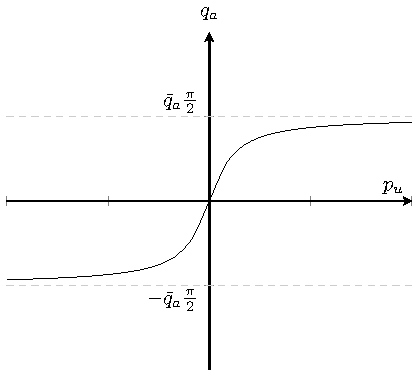
\includegraphics[width=0.7\linewidth]{qa_arctan.pdf}
    \caption{The acrobot constraint \(q_a = \bar{q}_a \arctan(I p_u)\).}
    \label{fig:qa-arctan}
\end{figure}

Recall that \((q_u, p_u)\) denote the angle and momentum of the acrobot's torso.
By Theorem \ref{thm:zero-dynamics}, the constrained dynamics arising from the
VNHC \eqref{eqn:acrobot-constraint} are parameterized fully by 
\((q_u,p_u) \in \SxR\).
Here, \eqref{eqn:g-qpu} reduces to
\begin{multline*}
    g(q_u,p_u) = \frac{
    (1+c_a)p_u}{ml^2(3+2c_a)}
    - \frac{mgl\bar{q}_a I (2-c_a^2)(2s_u + s_{ua})
    }{(3+2c_a)(1+I^2 p_u^2)}
    ,
\end{multline*}
and the constrained dynamics \eqref{eqn:qpu-dynamics} are
\begin{equation}\label{eqn:acrobot-constrained-dynamics}
    \begin{cases}
    \dot{q}_u &= \frac{(1+I^2 p_u^2)p_u + m^2gl^3\bar{q}_a I(2s_u + s_{ua})(1+c_a) }
            {ml^2(1+I^2 p_u^2)(3+2c_a)}
    ,    \\
    \dot{p}_u &= - m g l (2s_u + s_{ua})
    ,
    \end{cases}
\end{equation}
subject to \(q_a = \bar{q}_a \arctan(I p_u)\).

\subsection{Energy Injection and Dissipation with the Proposed VNHC}
Suppose for a moment that \(I = 0\) in \eqref{eqn:acrobot-constraint}, i.e.,
that the legs stay fully extended.
The acrobot becomes a nominal pendulum with two masses, whose total mechanical
energy is
\begin{equation}\label{eqn:nominal-energy}
    E(q_u,p_u) := \frac{p_u^2}{10ml^2} + 3mgl(1 - \cos(q_u))
    .
\end{equation}
The upright equilibrium of this pendulum is located at \((q_u,p_u) = (\pi,0)\).
Imagine the pendulum hits the bottom of the swing arc with momentum 
\(p_u \neq 0\). 
To reach the upright equilibrium, this momentum must be
\(p_u = \pm\sqrt{60m^2gl^3}\) because \(E(\pi,0) = E(0,\pm\sqrt{60m^2gl^3})\).
If the momentum is smaller in magnitude, the acrobot will oscillate; 
if it is larger, the pendulum will rotate around the bar.

When the pendulum is oscillating, its state \((q_u,p_u)\) lies in the set
\begin{equation}\label{eqn:oscillation-domain}
    \mathcal{O}_1 := \left\{(q_u,p_u) \in \SxR 
    \mid E(q_u,p_u) < E(\pi,0) \right\}
    ,
\end{equation}
which is shown in Figure \ref{fig:acrobot-oscillation-domain}.
If for some \(I \neq 0\) our VNHC injects energy into the acrobot on 
\(\mathcal{O}_1\), and the constrained dynamics escape
\(\mathcal{O}_1\) and hit the vertical line \(|q_u| = \pi\)
in finite time, then the acrobot is guaranteed to perform
giant-like motion and begin rotating around the bar.

When the pendulum is rotating with bounded momentum
\(\abs{p_u} < \rho\) (for some chosen \(\rho\)),
\((q_u,p_u)\) must lie inside the rotation domain
\begin{multline}\label{eqn:rotation-domain}
    \mathcal{R}(\rho) := \left\{
        (q_u,p_u) \in \SxR \mid\right.
        \\
        \left.E(\pi,0) < E(q_u,p_u) < E(0,\rho)
    \right\}
    .
\end{multline}
Connecting the regions \eqref{eqn:oscillation-domain} and
\eqref{eqn:rotation-domain} yields the set
\begin{equation}\label{eqn:o-rhobar}
    \mathcal{O}_2(\rho) := \left\{(q_u,p_u) \in \SxR
        \mid E(q_u,p_u) < E(0,\rho) \right\}
    ,
\end{equation}
shown in Figure \ref{fig:acrobot-o2}.
If the VNHC injects energy on \(\mathcal{O}_2(\rho)\) for some 
\(I \neq 0\), then the acrobot must necessarily swing up, begin rotating, 
and eventually rotate with a momentum of at least \(\rho\).

\begin{figure}
    \centering
    \begin{subfigure}[t]{0.45\linewidth}
        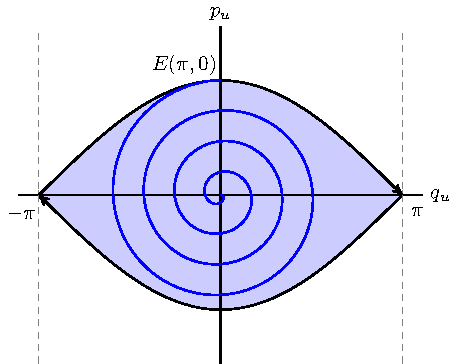
\includegraphics[width=\linewidth]{acrobot_oscillation_domain.pdf}
        \caption{The set \(\mathcal{O}_1\). An orbit starting in this set (blue)
            will pass through the level set \(E(\pi,0)\) of the nominal pendulum.}
        \label{fig:acrobot-oscillation-domain}
    \end{subfigure}
    \hfill
    \begin{subfigure}[t]{0.45\linewidth}
        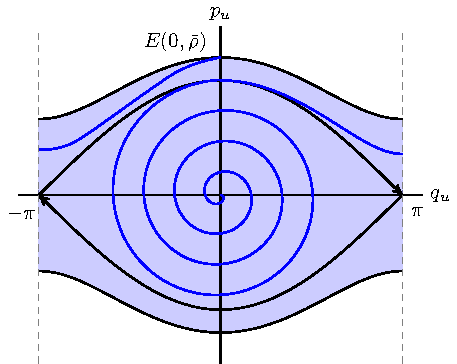
\includegraphics[width=\linewidth]{acrobot_omega.pdf}
        \caption{The set \(\mathcal{O}_2(\rho)\). Orbits starting in this
            set are guaranteed to reach the level set \(E(0,\rho)\) of the
            nominal pendulum.}
            \label{fig:acrobot-o2}
    \end{subfigure}
    \caption{The sets on which the acrobot gains energy, according to
        Theorem \ref{thm:acrobot-energy-stabilization}.}
\end{figure}

Unfortunately, our VNHC does not always inject energy on \(\mathcal{O}_1\) and
\(\mathcal{O}_2(\rho)\).
If \(I\) is too large, the leg controller saturates and the body oscillates
without gaining energy.
However, choosing \(I\) small enough guarantees the legs will synchronize
properly with the body, and the acrobot will begin rotating around the bar.
The following theorem provides conditions under which such an \(I\) exists.

\begin{thm}\label{thm:acrobot-energy-stabilization}
    Consider the acrobot with Hamiltonian dynamics given in
    \eqref{eqn:acrobot-hamiltonian}.
\begin{enumerate}
    \item For each \(m, g, l, \bar{q}_a > 0\), there exists
        \(I^\star > 0\) such that, for all \(I \in \, ]0,I^\star]\), the VNHC
        \eqref{eqn:acrobot-constraint} injects energy into the acrobot on
        \(\mathcal{O}_1\).
        Moreover, every orbit of the constrained dynamics 
        \eqref{eqn:acrobot-constrained-dynamics} will reach the line
        \(|q_u| = \pi\) in finite time.
        If instead \(I \in [-I^\star,0[\), the VNHC dissipates energy
        on \(\mathcal{O}_1\).
    \item Let \(C = m^2gl^3\bar{q}_a\) and 
        define \(b : \SxR_{> 0} \rightarrow \R\) by
    \[
        b(\beta,\rho_0) := 
        \frac{5C \left(
        \frac{C}{\bar{q}_a}\left(18s_\beta^2 + 30c_\beta(1 - c_\beta)\right)
            - c_\beta\rho_0^2
        \right)}{
        |\rho_0|\sqrt{\rho_0^2 - 30m^2gl^3(1 - c_\beta)}
        }
        .
    \]
        Define 
        \(S(\rho_0) := \int \limits_{0}^{2\pi} b(\sigma,\rho_0)d\sigma\).
        Fix \(\rho > \sqrt{60m^2gl^3}\) and
        suppose there exists \(\epsilon > 0\) so that 
        \(S(\rho_0) \geq \epsilon\) for all 
        \(\rho_0 \in \, \left]\sqrt{60m^2gl^3}, \rho\right]\).
        Then there exists \(I^{\star\star} \in \, ]0, I^\star]\) such that, for all 
        \(I \in \, ]0,I^{\star\star}]\), the VNHC
        \eqref{eqn:acrobot-constraint} injects energy into the acrobot on
        \(\mathcal{O}_2(\rho)\).
        If instead \(I \in [-I^{\star\star},0[\), the VNHC dissipates energy
        on \(\mathcal{O}_2(\rho)\).
\end{enumerate}
\end{thm}
\begin{proof}
    See Section \ref{sec:proof}.
\end{proof}

Notice that \(\mathcal{O}_1 \subset \mathcal{O}_2(\rho)\), yet
Theorem \ref{thm:acrobot-energy-stabilization} considers these sets separately.
This separation is advantageous because the first result holds for any positive
\(m\), \(g\), \(l\), and \(\bar{q}_a\). 
In other words, the first result of Theorem
\ref{thm:acrobot-energy-stabilization} states that all acrobots constrained by
\eqref{eqn:acrobot-constraint} will gain enough energy to begin rotating around
the bar.
%In the worst case, the acrobot will at least perform a swing-up routine to reach
%the unstable equilibrium at \((q_u,p_u) = (\pi,0)\).

For the acrobot to achieve giants with energy
\(E(0,\rho)\), it must satisfy the assumption on the integral
of \(b(\beta,\rho_0)\). 
The value of this integral depends on the acrobot's physical parameters.
If the assumption holds, there is some control value \(I\)
(which depends on \(\rho\)) for which the acrobot will 
achieve rotations with a momentum of at least \(\rho\).

\subsection{Energy Regulation}\label{sec:energy-reg}
One can apply the results of Theorem \ref{thm:acrobot-energy-stabilization} 
towards energy regulation; 
that is, one can stabilize oscillations or rotations by appropriately toggling
between injection and dissipation VNHCs, which can be achieved by changing the
sign of \(I\) in \eqref{eqn:acrobot-constraint}.
The acrobot is \textit{oscillating} when it swings back and forth without
performing a full revolution around the pivot point.
Oscillations correspond to \(p_u\) changing sign periodically, and the peak
torso angle (i.e., the point where an orbit crosses the \(q_u\)-axis)
is called the \textit{oscillation angle}.
Conversely, the acrobot is \textit{rotating} when its torso is performing full
revolutions around the pivot, which corresponds mathematically to \(p_u\)
maintaining the same sign.
The momentum achieved by the acrobot at the bottom of the swing
(i.e., the point where an orbit of rotation crosses the \(p_u\)-axis) is
called the \textit{rotation rate}.

\textbf{Rotation Regulation}: one chooses a desired rotation rate 
\(p_\text{des} > 0\) and a hysteresis value \(\delta \in [0,1]\).
Each time the orbit crosses the \(p_u\)-axis (i.e. when \(q_u = 0\)), the
supervisor changes which VNHC is enforced as follows:
\begin{itemize}
    \item If \(|p_u| < (1-\delta)p_\text{des}\), enable the injection VNHC by
        setting \(I > 0\) in \eqref{eqn:acrobot-constraint}.
    \item If \(|p_u| > (1+\delta)p_\text{des}\), enable the dissipation VNHC by
        replacing \(I > 0\) with \(-I < 0\) in \eqref{eqn:acrobot-constraint}.
    \item If \((1-\delta)p_\text{des} \leq |p_u| \leq (1+\delta)p_\text{des}\),
        extend the leg fully by setting \(q_a = 0\).
        For these simulations, we assume this can be done instantaneously,
        though in practice this is impossible.
\end{itemize}
Note that all orbits of the acrobot must cross the \(p_u\) axis, 
so this method will stabilize a rotation even if the acrobot is initialized in
\(\mathcal{O}_1\).
Also, the above supervisor is designed to regulate a rotation rate, but it
cannot regulate the rotation direction.

The term ``rotation regulation" implies that one must choose
\(p_\text{des}\) and \(\delta\) so that 
\((1-\delta) p_\text{des} > \sqrt{60m^2gl^3}\).
In fact, it is entirely possible to choose \(p_\text{des}\) and \(\delta\) so
that \((1+\delta)p_\text{des} \leq \sqrt{60m^2gl^3}\).
Rather than stabilizing a rotation, the supervisor would then stabilize an
oscillation whose momentum at the bottom of the swing arc is \(p_\text{des}\).
However, there is a preferred method for stabilizing oscillations
which we outline next.

\textbf{Oscillation Regulation}: one chooses a desired oscillation angle 
\(q_\text{des} \in \, ]0,\pi[\) and, to avoid infinite switching, a
hysteresis value \(\delta \in [0,\pi/q_\text{des} - 1]\).
An orbit in the \((q_u,p_u)\)-plane will either cross the \(q_u\) axis if the
orbit corresponds to a rocking motion, or it will cross the line \(|q_u| = \pi\)
if the orbit corresponds to a full revolution.
When either of these occur, the supervisor does the following: 
\begin{itemize}
    \item If \(|q_u| < (1-\delta)q_\text{des}\), enable the injection VNHC.
    \item If \(|q_u| > (1+\delta)q_\text{des}\), enable the dissipation VNHC.
    \item If \((1-\delta)q_\text{des} \leq |q_u| \leq (1+\delta)q_\text{des}\),
        keep the leg extended at \(q_a = 0\). This can be done continously since
        \(q_a = 0\) when \(p_u = 0\).
\end{itemize}
Note that by our choice of \(\delta\), if the supervisor kicks in when 
\(|q_u| = \pi\) (i.e., when the robot is rotating) then the supervisor will
automatically enable the dissipation VNHC.

%/========== Experiments ==========/%
\section{Simulation Results}\label{sec:simulations}
In Section \ref{sec:experiments} we will test our VNHC on a physical acrobot.
%built by Xingbo Wang \cite{xingbo_thesis}.
This acrobot cannot be modelled by the simplified setup in Figure
\ref{fig:acrobot}, because the torso and leg links have 
distributed mass. 
We must therefore use the more general acrobot model in Figure
\ref{fig:acrobot-model} to represent this system.
Let us define 
\begin{align*}
    m_{11}(q) := &m_a l_u^2 + 2m_al_ul_{c_a}\cos(q_a) + m_al_{c_a}^2 +
    m_ul_{c_u}^2 \\
                 &+ J_u + J_a
                 , \\
    m_{12}(q) := &m_al_{c_a}^2 + m_al_ul_{c_a}\cos(q_a) + J_a
    , \\
    m_{22}(q) := &m_al_{c_a}^2 + J_a,
\end{align*}
where \(J_u\) and \(J_a\) are the moments of inertia of the torso and leg links
respectively. 
The general acrobot has inertia matrix
\begin{equation*}
    M(q) = \begin{bmatrix}
        m_{11}(q) & m_{12}(q) \\
        m_{12}(q) & m_{22}(q)
    \end{bmatrix}
    ,
\end{equation*}
and potential function
\begin{equation*}
    V(q) = g\big(m_al_{c_a}(1-c_{ua})
    + (m_al_u + m_ul_{c_u})(1-c_u)\big)
    .
\end{equation*}

\begin{figure}
    \centering
    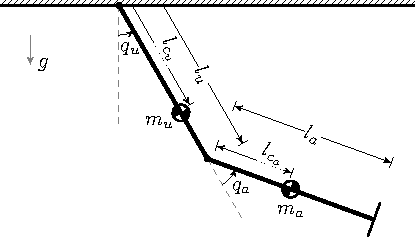
\includegraphics[width=0.8\linewidth]{acrobot_model.pdf}
    \caption{The general acrobot model, represented by two weighted rods
    differing in both length and mass.}%
    \label{fig:acrobot-model}
\end{figure}

Recall that we defined the sets \(\mathcal{O}_1\) and
\(\mathcal{O}_2(\rho)\) used in Theorem \ref{thm:acrobot-energy-stabilization}
via the mechanical energy \eqref{eqn:nominal-energy} of the nominal
pendulum associated with a simplified acrobot.
We obtained this nominal pendulum by setting \(I = 0\) in
\eqref{eqn:acrobot-constraint}.
The boundary between oscillations and rotations of the nominal
pendulum is obtained by finding the level set \(E_\pi\) of the nominal energy
corresponding to the upright equilibrium \((q_u,p_u) = (\pi,0)\).

We can extend this idea to find the nominal pendulum associated with our
physical acrobot, whose parameters are provided in Table
\ref{tab:acrobot-parameters}.
Setting \(I = 0\) in \eqref{eqn:acrobot-constraint} for this acrobot
yields the following mechanical energy of the nominal pendulum:
\[
    E(q_u,p_u) \approx 396.5501 p_u^2 + 0.5997(1 - \cos(q_u))
    .
\]
Despite the change in model, the level set \(E_\pi\) with energy 
\(E(\pi,0)\) remains the boundary between oscillations and rotations
for this nominal pendulum.

We will now simulate the effects of constraining our real acrobot with the VNHC
\eqref{eqn:acrobot-constraint}, thereby demonstrating that VNHCs are robust to
model mismatch.
According to Theorem \ref{thm:acrobot-energy-stabilization}, the control
parameter \(I\) must be ``small" for our VNHC to inject (or dissipate) energy
into the simplified acrobot. 
Unfortunately, the Theorem does not specify how small \(|I|\) must be;
while we could make it arbitrarily small in simulations, we will eventually
implement this VNHC on a physical testbed where \(|I|\) must be large enough to
overcome friction.

Setting \(\bar{q}_a = 1\), we experimentally determined that \(|I| = 10\) is a
viable control parameter, so this is the value we will use for all simulations
and experiments.
In other words, our \textit{injection VNHC} is \eqref{eqn:acrobot-constraint} with 
\(I = 10\) while our \textit{dissipation VNHC} is \eqref{eqn:acrobot-constraint} with 
\(I = -10\).

\begin{table}
    \centering
    \caption{Physical parameters for the real acrobot.}
    \label{tab:acrobot-parameters}
    \resizebox{\columnwidth}{!}{%
    \begin{tabular}{ccccccccc}
        \toprule
        $m_u$ & $m_a$ & $l_u$ & $l_a$ & $l_{c_u}$ & $l_{c_a}$ & $J_u$ & $J_a$ & $g$ \\
        (kg) & (kg) & (m) & (m) & (m) & (m) & (kg\(\cdot\)m\(^2\)) &
        (kg\(\cdot\)m\(^2\)) & (m/s\(^2\)) \\
        \midrule
        0.2112 & 0.1979 & % mass
        0.148 & 0.145 & % total length
        0.073 & 0.083 & % COM distance
        0.00129 & 0.00075 & % moment of inertia
        9.81 \\ % gravity
        \bottomrule
    \end{tabular}
    } % resizebox
\end{table}

\subsection{Energy Injection}

In simulation, we stabilized the injection VNHC for the acrobot using the
controller \eqref{eqn:stabilizing-controller}.
We initialized the acrobot on the constraint manifold
with initial condition \((q_u,p_u) = \left(\pi/32,0 \right)\) and simulated the
constrained system for \(30\) seconds.
The resulting orbit is plotted in Figure
\ref{fig:acrobot-in-orbit}.

The level set \(E_\pi\) with energy \(E(\pi,0)\) is outlined in black.
Recall that this level set is the boundary between oscillations and rotations of the
nominal pendulum.
The points where the orbit exits \(E_\pi\) are marked with black asterisks,
with the final departure marked by a red asterisk.
Interestingly, our choice of \(I\) is large enough that we observe significant
differences between the nominal pendulum and the constrained dynamics:
\(E_\pi\) intersects the \(p_u\)-axis at \(\abs{p_u} \approx 0.17\), yet the
constrained acrobot begins rotating once it hits the
\(p_u\)-axis at \(\abs{p_u} \approx 0.16\). 
This indicates that higher values of \(I\) enable the acrobot to gain energy
faster and begin rotating sooner, so long as the actuator does not saturate.

\begin{figure}[]
    \centering
    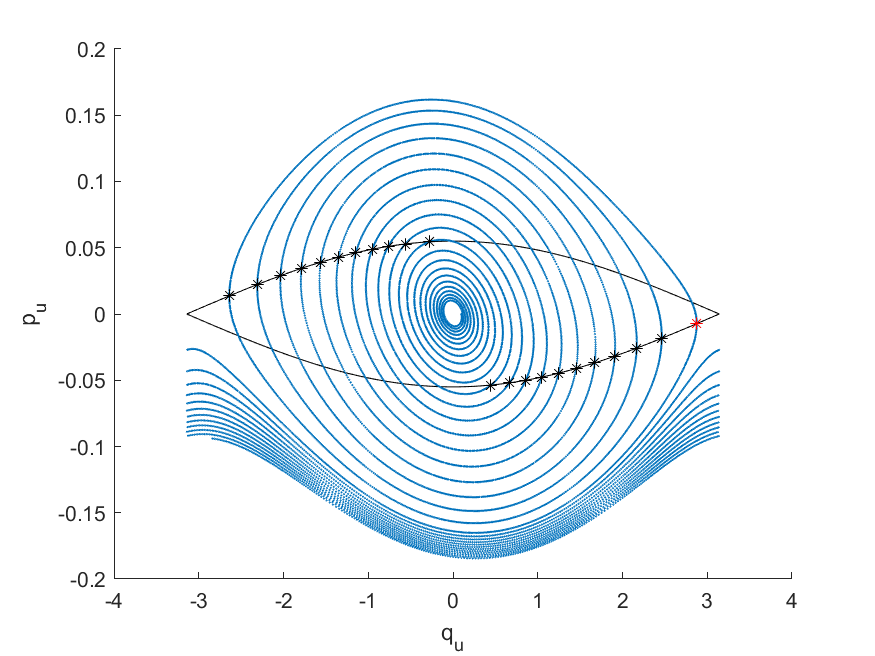
\includegraphics[width=0.8\linewidth]{acrobot_in_orbit.png}
    \caption{A simulation of the acrobot gaining energy.}
    \label{fig:acrobot-in-orbit}
\end{figure}

To verify numerically that the acrobot would consistently achieve rotations, we
ran a Monte-Carlo \cite{montecarlo} simulation where we initialized the acrobot
randomly inside the sublevel set
\[
    \left\{(q_u,p_u) \in \SxR \mid
    E(q_u,p_u) \leq E\left(\frac{\pi}{32},0\right)\right\}
    ,
\] 
and measured how long it took to begin rotating.
The results in Figure \ref{fig:acrobot-mc} show that
the acrobot always rotated within 20--40 seconds.

\begin{figure}[]
    \centering
    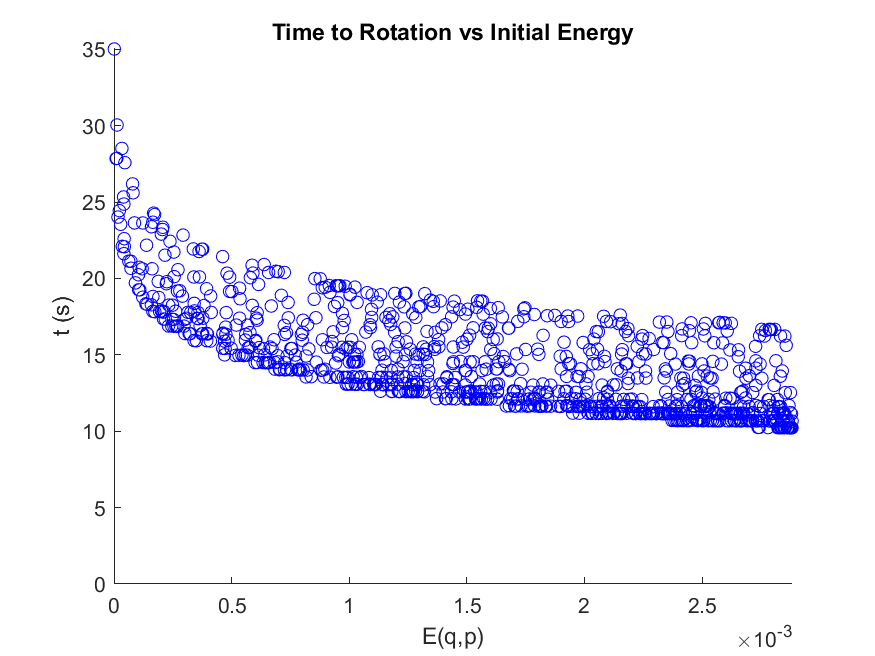
\includegraphics[width=0.8\linewidth]{acrobot_mc.png}
    \caption{Monte Carlo simulation for energy injection.}
    \label{fig:acrobot-mc}
\end{figure}

\subsection{Energy Dissipation}

In simulation, we stabilized the dissipation VNHC and initialized the acrobot on
the constraint manifold with a rotation \((q_u,p_u) = (0,0.18)\).
We simulated the constrained system for \(30\) seconds and plotted the
resulting orbit in Figure \ref{fig:acrobot-diss-orbit}. 
As expected, the acrobot slows down over time.
We highlight the locations where the orbit crossed the set \(E_\pi\) by
black asterisks, with the final crossing in red.
After this final crossing, the acrobot ceased rotating and its oscillations
decayed to zero.

\begin{figure}
    \centering
    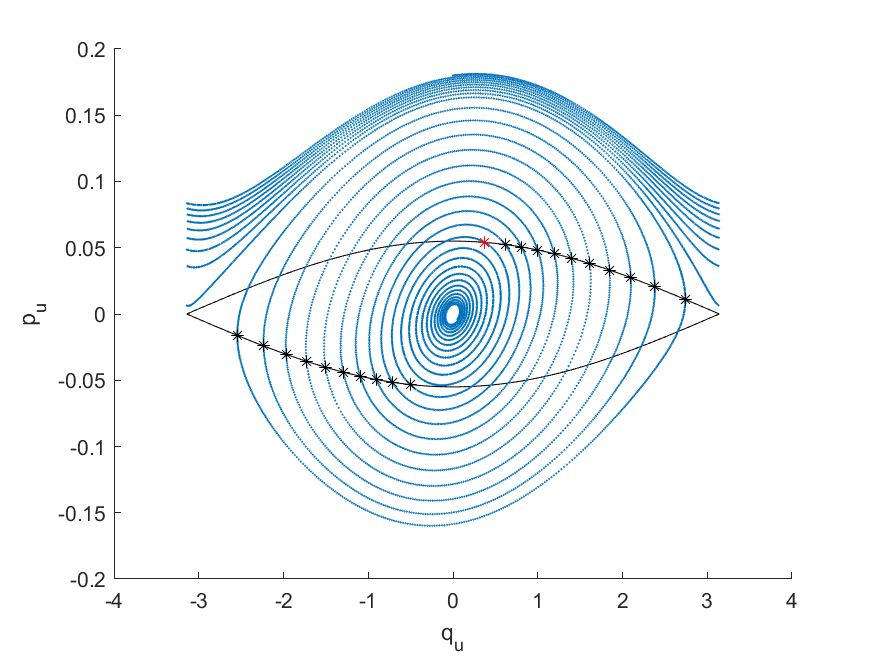
\includegraphics[width=0.8\linewidth]{acrobot_diss_orbit.png}
    \caption{A simulation of the acrobot dissipating energy.}
    \label{fig:acrobot-diss-orbit}
\end{figure}

\subsection{Oscillation Regulation}

Recall from Section \ref{sec:energy-reg} that one can use a supervisor to stabilize
oscillations by appropriately toggling between injection and dissipation VNHCs
whenever the orbit of the acrobot crosses the \(q_u\)-axis.
Figure \ref{fig:acrobot-osc-reg} shows the supervisor stabilizing an
oscillation with body angle \(q_\text{des} = \pi/2\) and a 
\(5\%\) hysteresis, meaning \(\delta = 0.05\).
The supervisor reevaluated its choice of VNHC at each black asterisk;  
the red contour corresponds to the part of the orbit where the supervisor kept
the leg extended, because the oscillation was within tolerance of
\(q_\text{des}\).
The solid black line is the desired oscillation, and the dashed black
lines show the hysteresis around that orbit.

In Figure \ref{fig:acrobot-osc-reg-in} the acrobot was initialized at 
\((q_u,p_u) = (\pi/32,0)\); here the supervisor injected energy to stabilize the
desired orbit.
In Figure \ref{fig:acrobot-osc-reg-diss} the acrobot was initialized at the rotation
\((q_u,p_u) = (0,0.19)\); note that the supervisor is first enabled at the line
\(|q_u| = \pi\) and dissipates energy. Eventually the acrobot begins a rocking
motion and the supervisor is enable again each time the acrobot hits the
\(q_u\)-axis. 
The supervisor continues to dissipate energy until it stabilizes the desired
oscillation.

\begin{figure}
    \centering
    \begin{subfigure}[t]{0.49\linewidth}
        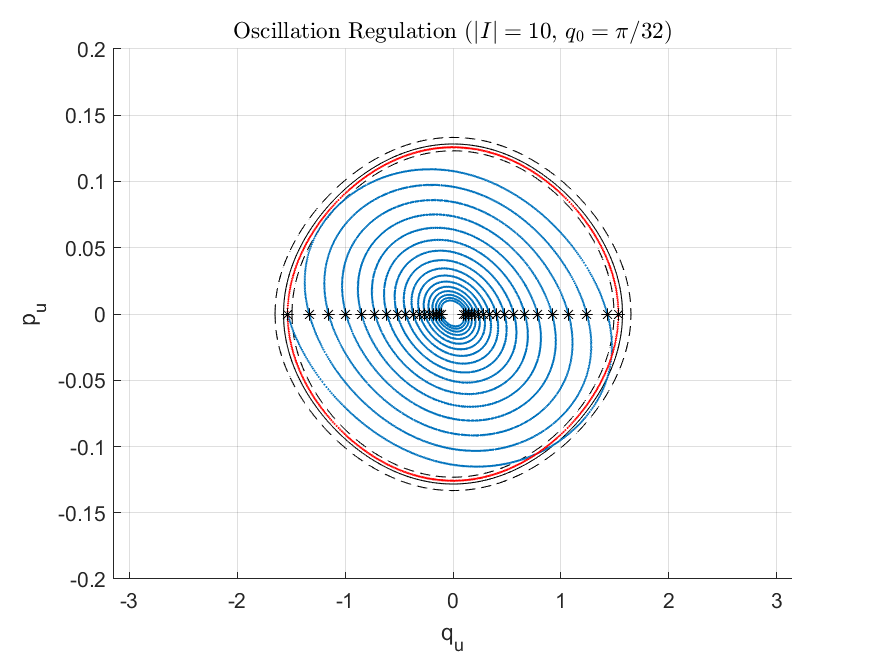
\includegraphics[width=\linewidth]{acrobot_osc_orbit_1.png}
        \caption{Stabilizing an oscillation from below.}
        \label{fig:acrobot-osc-reg-in}
    \end{subfigure}
    \begin{subfigure}[t]{0.49\linewidth}
        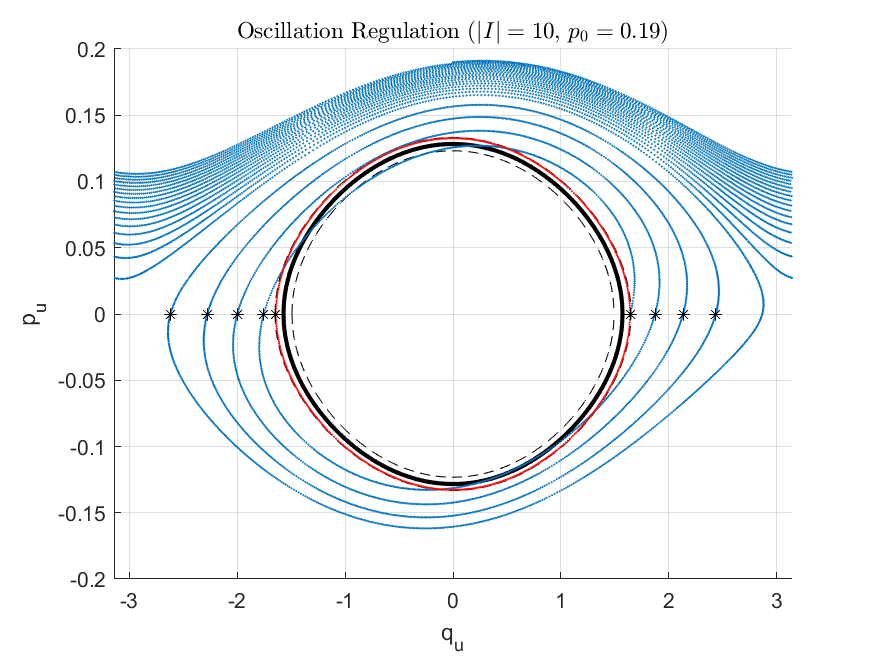
\includegraphics[width=\linewidth]{acrobot_osc_orbit_2.png}
        \caption{Stabilizing an oscillation from above.}
        \label{fig:acrobot-osc-reg-diss}
    \end{subfigure}
    \caption{Using a supervisor to stabilize the oscillation with peak angle
    \(q_\text{des} = \pi/2\). The desired oscillation is depicted with a solid
    black line.}
    \label{fig:acrobot-osc-reg}
\end{figure}

\subsection{Rotation Regulation}
One can also use a supervisor to stabilize rotations through the mechanism
described in Section \ref{sec:energy-reg}, where the supervisor toggles between
injection and dissipation VNHCs at each crossing of the \(p_u\)-axis.
Rotation regulation for the acrobot is demonstrated in 
Figure \ref{fig:acrobot-rot-reg}, where the supervisor stabilizes 
\(p_\text{des} = 0.19\) with a \(2\%\) hysteresis \(\delta = 0.02\).
The supervisor evaluated its choice of VNHC at each black asterisk.
Once it was within range of \(p_\text{des}\) it extended the legs completely,
the orbit of which is shown in red.

In Figure \ref{fig:acrobot-rot-reg-in} the acrobot was initialized at 
the oscillation \((q_u,p_u) = (\pi/2,0)\); here the supervisor injected energy
until the orbit hit the \(p_u\)-axis near \(p_\text{des}\).
In Figure \ref{fig:acrobot-rot-reg-diss} the acrobot was initialized at the
(fast) rotation \((q_u,p_u) = (0, 0.23)\); here the supervisor dissipated energy.
In both cases, the desired rotation was stabilized correctly.

\begin{figure}
    \centering
    \begin{subfigure}[t]{0.49\linewidth}
        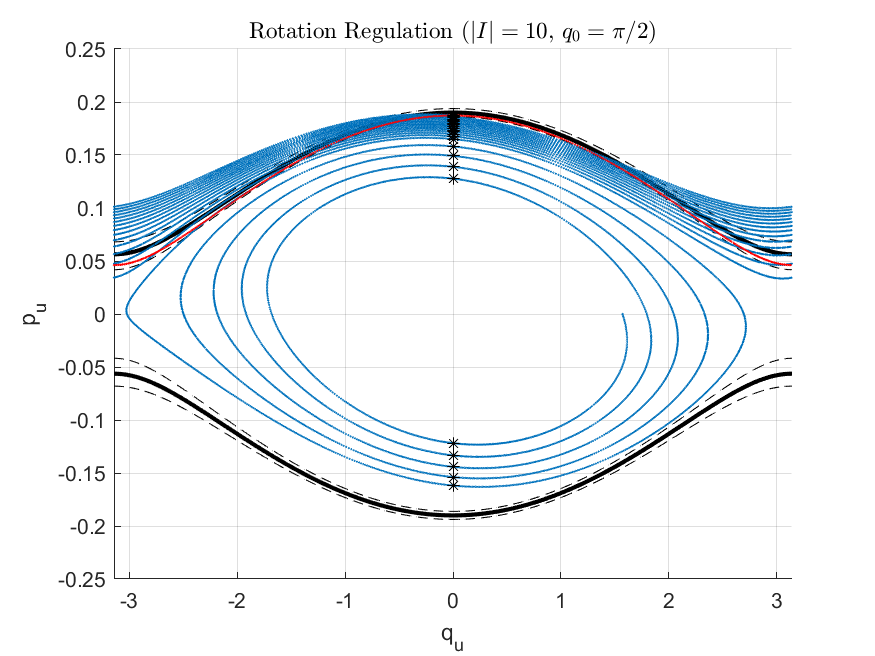
\includegraphics[width=\linewidth]{acrobot_rot_orbit_1.png}
        \caption{Stabilizing a rotation from below.}
        \label{fig:acrobot-rot-reg-in}
    \end{subfigure}
    \begin{subfigure}[t]{0.49\linewidth}
        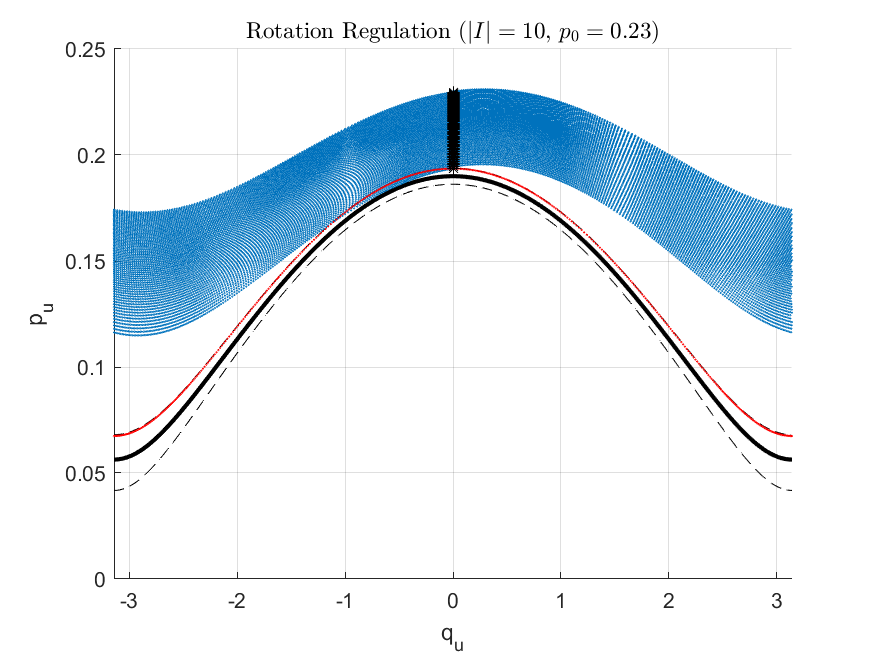
\includegraphics[width=\linewidth]{acrobot_rot_orbit_2.png}
        \caption{Stabilizing a rotation from above.}
        \label{fig:acrobot-rot-reg-diss}
    \end{subfigure}
    \caption{Using a supervisor to stabilize the rotation with maximal momentum
    \(p_\text{des} = 0.23\). The desired rotation is depicted with a solid black
    line.}
    \label{fig:acrobot-rot-reg}
\end{figure}

Note the difference in shape between the blue rotations of the dissipation VNHC
and the red rotation of the nominal pendulum in Figure
\ref{fig:acrobot-rot-reg}: the red one slows down much more
near \(|q_u| = \pi\).
This difference arises because of the size of \(I\):
if \(|I|\) were smaller, the blue rotations would be more similar in shape to the
red one because the constrained dynamics for the dissipation VNHC would be
well approximated by the nominal pendulum.

\subsection{Summary of Results}
The simulation results in this section demonstrate the energy regulation
capabilities of our VNHC.  
We were able to stabilize both oscillations and rotations by implementing a
control supervisor which toggled between injection, dissipation, and
leg-extension VNHCs.
In particular, these simulations indicate that our VNHC
works even for acrobots whose limbs have differing masses and lengths.

\section{Physical Experiments}\label{sec:experiments}

\subsection{Hardware Description}
In this section we will demonstrate that our VNHC is robust to friction, sensor
noise, and other real-world considerations by testing it on our physical
acrobot (Figure \ref{fig:xingbo-acrobot}).
This platform is called SUGAR, which stands for
Simple Underactuated Gymnastics and Acrobatics Robot.
Its dynamic parameters are outlined in Table \ref{tab:acrobot-parameters}.


\begin{figure}
    \centering
    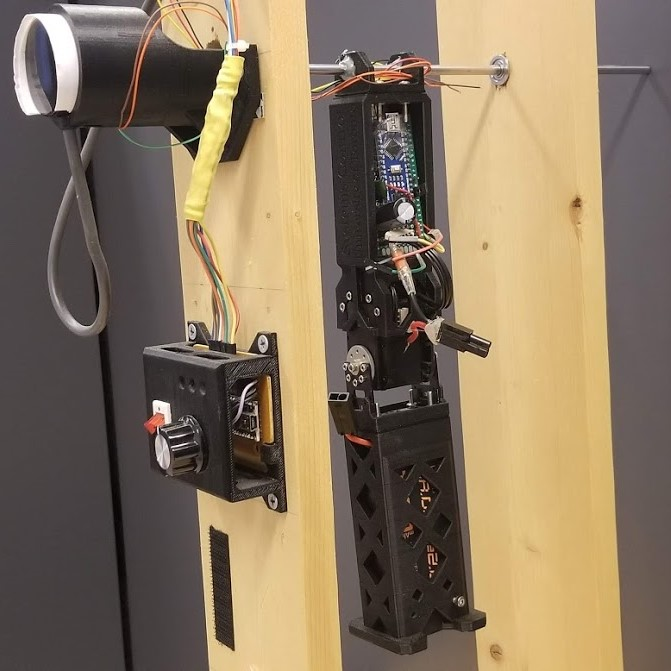
\includegraphics[width=0.9\linewidth]{xingbo_acrobot.jpg}
    \caption{SUGAR is the physical acrobot built by Wang \cite{xingbo_thesis}.}
    \label{fig:xingbo-acrobot}
\end{figure}

SUGAR is comprised of two 3D-printed links: a torso and a leg.
The torso houses an Arduino Nano microcontroller unit (MCU) which controls
a Dynamixel RX24F servo motor between the torso and the leg.
The MCU and the motor are powered by a 12V battery held in a compartment
in the leg.

The torso is rigidly attached to a metal bar, which is held up by two wooden
posts.
On the exterior of one post is a control box with a power switch and a second
Arduino Nano 328.
The purpose of this control box is to read measurements from a rotary
encoder connected to the metal bar, and to transmit these measurements to the
MCU.
The two Arduinos communicate through wires attached to a slip ring on the metal
bar, and the signals are transmitted via I2C.
The control box also provides a USB interface which allows the user to read the
data from the acrobot in real time.

The rotary encoder directly measures \(q_u\), and the Dynamixel servo
motor provides measurements of \(q_a\).
However, there are no sensors measuring the velocity \(\dot{q}\), which means we cannot
directly evaluate \(p_u\) and \(p_a\).
To resolve this issue, the MCU estimates \(\dot{q}\) by applying a washout
filter to sequential measurements of \(q\).
We then compute \(p = M(q)\dot{q}\) for use in the VNHC controller.

The communication speed between Arduinos restricts the sampling rate of \(p\) to
500Hz.
This low sampling rate results in a noisy momentum signal which suffers
from noticeable phase lag.
This also rate-limits the control signal to \(500\)Hz, which impacts any control
implementation.

Finally, The Dynamixel servo motor does not have a torque control mode; instead,
we can assign the servo setpoint at iteration \(k \in \mathbb{Z}_{> 0}\)
via \(q_a^{k} = \arctan(I p_u^{k-1})\).
This negatively affects the stabilization to the constraint
manifold because we are introducing timing errors from the servo's built-in PID
controller.

\subsection{Experimental Results}

We performed the following tests on SUGAR with the energy injection VNHC.

\begin{enumerate}
    \item \textbf{Baseline Test:} 
    we initialized SUGAR at 
    \((q_u,p_u) \approx \left(\pi/8,0\right)\). 
    The resulting orbit in Figure \ref{fig:acrobot-unperturbed-orbit} shows
    that SUGAR clearly gaining energy over time.
    Its motion looks similar to that of the energy injection simulation (Figure
    \ref{fig:acrobot-in-orbit}), though its energy gain ceases once it reaches a
    rotation with energy \(E(0,0.195)\).
    The energy gain likely ceases because of friction at the pivot, which was
    not modelled in simulation.

\begin{figure}
    \centering
    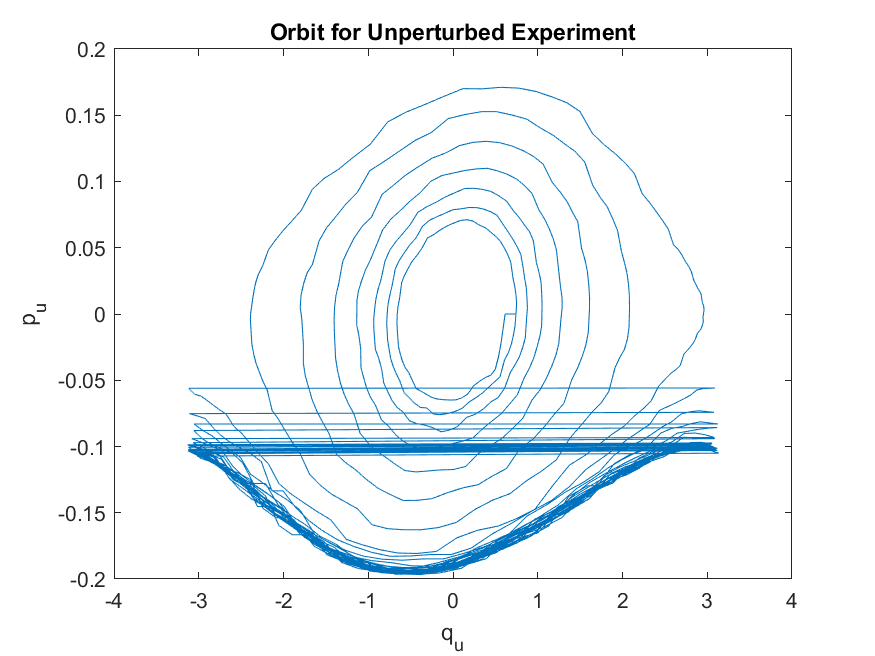
\includegraphics[width=0.8\linewidth]{acrobot_unperturbed_orbit.png}
    \caption{Baseline Test: SUGAR's baseline energy injection orbit.}
    \label{fig:acrobot-unperturbed-orbit}
\end{figure}

\item \textbf{Perturbation Test 1:}
    we initialized SUGAR at 
    \((q_u,p_u) \approx \left(\pi,0\right)\), let it run for 15
    seconds, then introduced a rod as SUGAR passed through the bottom of
    its arc.
    This caused a collision which stopped SUGAR in its tracks, at which
    point we immediately removed the rod so SUGAR could continue
    unperturbed.
    The resulting orbit is shown in Figure \ref{fig:acrobot-stopped-orbit}.
    The blue rotation curve corresponds to the orbit before the disturbance,
    while the red spiral confirms that SUGAR begins oscillating after it
    was stopped.  
    After the collision, SUGAR gains energy and eventually starts
    rotating again.

\begin{figure}
    \centering
    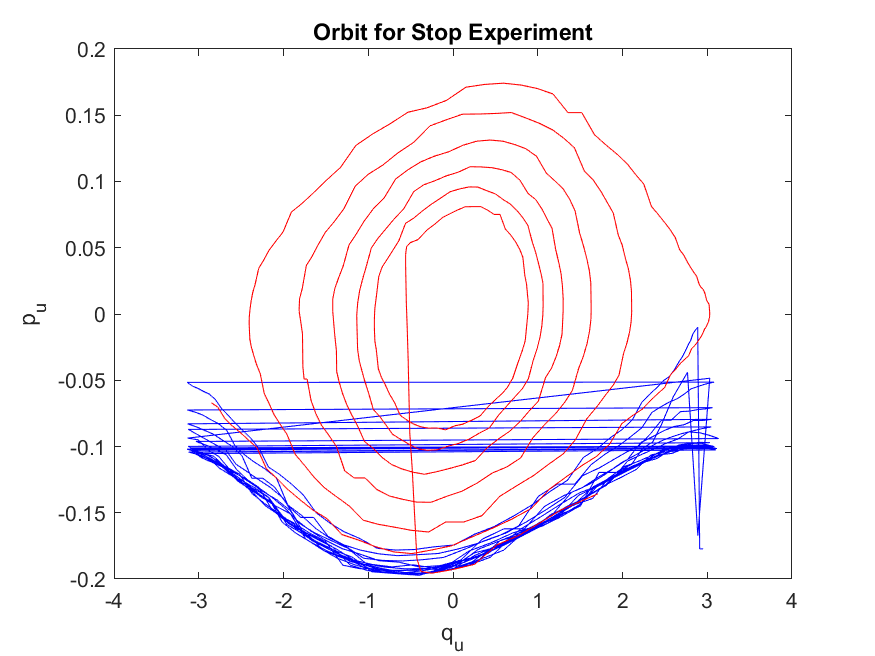
\includegraphics[width=0.8\linewidth]{acrobot_stopped_orbit.png}
    \caption{Perturbation Test 1: SUGAR's orbit before (blue) and after (red) stopping.}
    \label{fig:acrobot-stopped-orbit}
\end{figure}


\item \textbf{Perturbation Test 2:}
    to see how SUGAR would respond when pushed, we allowed
    it to rotate unperturbed for 15 seconds and then pushed it in its
    direction of motion.
    The orbit in Figure \ref{fig:acrobot-fpush-orbit} shows that SUGAR,
    when pushed, rotates with energy \(E(0,-0.22)\), but then slows down until
    it reaches a rotation with energy \(E(0,-0.195)\).
    We repeated this test by pushing SUGAR against its direction of motion.
    The orbit in Figure \ref{fig:acrobot-rpush-orbit} demonstrates that SUGAR
    readily changes direction, and quickly achieves its maximum speed
    with energy \(E(0,0.195)\).
\end{enumerate}

In simulation, the acrobot was able to gain energy even when initialized
with energy \(E(q_u,p_u) > E(0,0.195)\). 
The baseline and push tests suggest that our VNHC injects energy into SUGAR
only on \(\mathcal{O}_2(0.195)\).
This difference between simulation and implementation is likely due to
friction, as well as timing errors incurred by the PID controller in the servo
motor.

\begin{figure}
    \centering
    \begin{subfigure}[ht]{0.49\linewidth}
        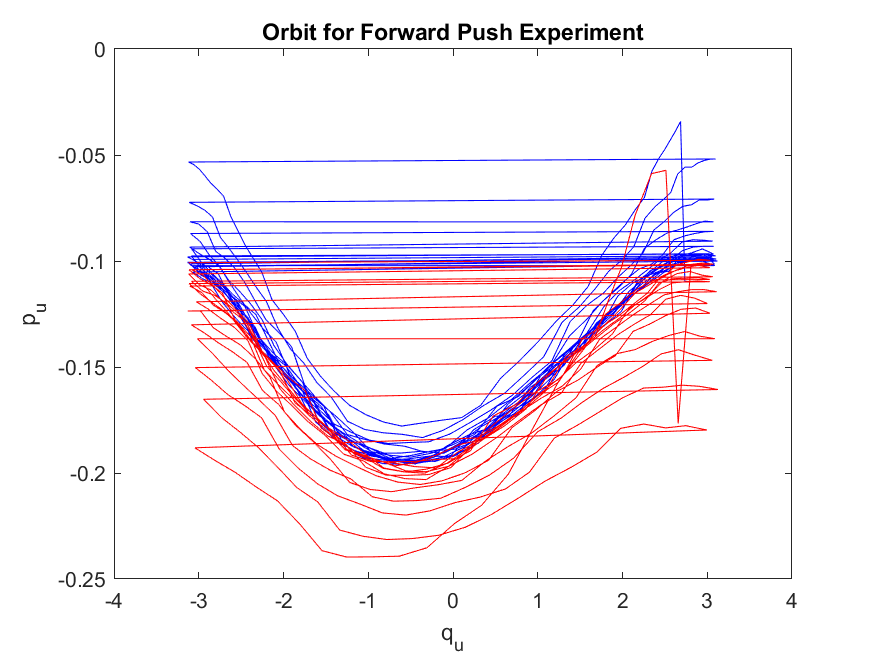
\includegraphics[width=\linewidth]{acrobot_fpush_orbit.png}
        \caption{The forwards push test.}
        \label{fig:acrobot-fpush-orbit}
    \end{subfigure}
    \begin{subfigure}[ht]{0.49\linewidth}
        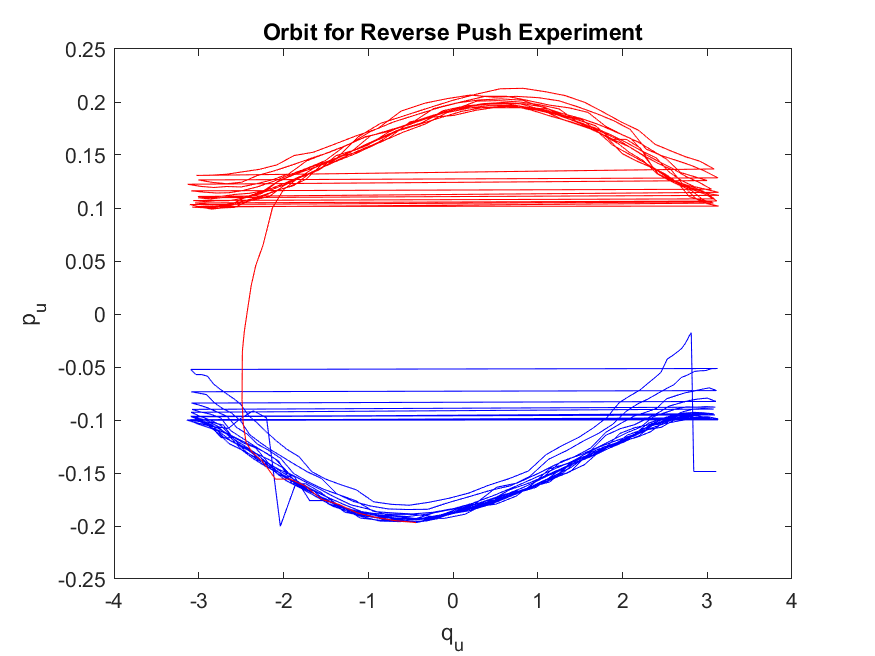
\includegraphics[width=\linewidth]{acrobot_rpush_orbit.png}
        \caption{The reverse push test.}
        \label{fig:acrobot-rpush-orbit}
    \end{subfigure}
    \caption{Perturbation Test 2: SUGAR's orbit before (blue) and after (red) pushing.}
\end{figure}

\subsection{Summary of Results} 
We performed three tests on SUGAR: a baseline energy injection test,
a stop test, and a push test.
These experiments demonstrate that VNHC-based energy injection is robust to
significant model mismatch, friction, sensor noise, discretized control
implementation, rate-limited measurement and control signals, and dramatic
external disturbances.

%/========== Proof ==========/%
\section{Proof of Theorem \ref{thm:acrobot-energy-stabilization}}\label{sec:proof}
In this section we prove Theorem \ref{thm:acrobot-energy-stabilization},
which claims the acrobot gains/loses energy on \(\mathcal{O}_1\) and
\(\mathcal{O}_2(\rho)\).
These are the sublevel sets \eqref{eqn:oscillation-domain} and
\eqref{eqn:o-rhobar} of the nominal pendulum's energy \(E(q_u,p_u)\) defined in
\eqref{eqn:nominal-energy}.

Here is fundamental idea behind this proof:
for each of \(\mathcal{O}_1\) or \(\mathcal{O}_2(\rho)\),
we can find a diffeomorphism \(T(q_u,p_u) = (r,\theta)\) into pseudo-polar
coordinates adapted to level sets of \(E(q_u,p_u)\);
that is, when \(I = 0\) in \eqref{eqn:acrobot-constraint}, the pseudo-radius
\(r\) chooses a level set of \(E\) and the pseudo-angle \(\theta\) chooses a
point on that level set.
If the constrained dynamics in \((r,\theta)\) coordinates flow in such a way
that \(r\) increases ``on average", then \(E\) must also increase ``on average",
and the original constrained dynamics \eqref{eqn:acrobot-constrained-dynamics} 
must be gaining energy on the domain of the diffeomorphism.

The following lemma provides a set of conditions on the \((r,\theta)\) dynamics
under which energy will increase on a domain \(D\); later in this section, we
will assign \(D = \mathcal{O}_1\) or \(D = \mathcal{O}_2(\rho)\), find an
appropriate transformation \(T\), and apply this lemma to prove the claims in
Theorem \ref{thm:acrobot-energy-stabilization}.

%Here is the summary of this proof: for certain subsets
%\(D \subset \SxR\), one can find a change of coordinates into 
%pseudo-polar coordinates adapted to level sets of \(E(q_u,p_u)\)
%(see the general procedure devised by Mohammadi \etal 
%\cite{dynamic_vhcs_stabilize_closed_orbits}).
%That is, when \(I = 0\) in \eqref{eqn:acrobot-constraint}, one can find
%a diffeomorphism \(T(q_u,p_u) =  (r,\theta)\), where \(r\)
%chooses a level set of \(E\) and \(\theta\) chooses a point on that level set.
%The acrobot's dynamics in \((r,\theta)\) coordinates will satisfy 
%\(\dot{r} = 0\) and \(\dot{\theta} > 0\) when \(I = 0\).
%By continuity of the constrained dynamics with respect to \(I\),
%we maintain \(\dot{\theta} > 0\) for small non-zero values of \(I\).
%This will enable us to perform a time-scaling transformation 
%\(t = t(\theta)\), and study how the acrobot's pseudo-radius \(r\) evolves as a
%function of the pseudo-angle \(\theta\), rather than as a function of time.
%We will formally show that \(r(\theta)\) increases on average, which means
%\(E\) also increases on average.
%This in turn implies the constrained dynamics are gaining energy on \(D\).
%We formalize these ideas in the following lemma.

\begin{lemma}\label{lemma:energy-regulation-D}
    Consider the simplified acrobot \eqref{eqn:acrobot-hamiltonian} constrained
    by the VNHC \eqref{eqn:acrobot-constraint}, whose constrained dynamics are
    \eqref{eqn:acrobot-constrained-dynamics}.
    Let \(D \subset \SxR\) be open and 
    let \(]\underline{r}, \overline{r}[ \, \subset \R_{> 0}\).
    Suppose there exists a diffeomorphism 
    \begin{align*}
        T : D &\to ]\underline{r},\overline{r}[ \, \times \Sone
         \\
        (q_u,p_u) &\mapsto (r,\theta)
        ,
    \end{align*}
    yielding the new constrained dynamics \(\dot{r} = f_r(\theta,r,I)\),
    \(\dot{\theta} = f_\theta(\theta,r,I)\).
    Suppose that \(f_r(\theta,r,0) \equiv 0\) and \(f_\theta(\theta,r,0) > 0\).
    Let \(g(\theta,r,I) = f_r(\theta,r,I)/f_\theta(\theta,r,I)\), and assume that 
    \((\partial g/\partial r)(\theta,r,0) \equiv 0\) and
    \(b(\theta,r) := (\partial g/\partial I)(\theta,r,0)\)
    is \(2\pi\)-periodic in \(\theta\).
    Assume also that there exists \(\epsilon > 0\) such that 
    \(S(r_0) := \int_0^{2\pi} b(\sigma,r_0)d\sigma \geq \epsilon\)
%    \[
%        S(r_0) := \int \limits_0^{2\pi} b(\sigma,r_0)d\sigma \geq \epsilon
%        ,
%    \]
    for all \(r_0 \in \, ]\underline{r},\overline{r}[\).
    Then there exists \(I^\star > 0\) small enough that the constrained dynamics
    gain energy on \(D\) for all \(I \in \,]0, I^\star]\), and lose energy on \(D\)
    for all \(I \in [-I^\star, 0[\).
\end{lemma}
\begin{proof}
    Since \(\dot{\theta} > 0\) when \(I = 0\) and the constrained dynamics 
    in \((r,\theta)\) coordinates are continuous in \(I\), there exists 
    \(I_1 > 0\) small enough that \(\dot{\theta} > 0\) for all
    \(I \in \, [-I_1,I_1]\).
    Hence, we can perform a time reparameterization \(t = t(\theta)\) to get a
    time-scaled pseudo-radius \(\hat{r}(\theta) := r(t(\theta))\).
    This reduces the system \((\dot{r},\dot{\theta})\) into the scalar
    time-varying ODE
    \begin{equation}\label{eqn:rhat-ode}
        \begin{cases}
            \hat{r}^\prime= \left.\frac{dr}{dt} \frac{dt}{d\theta}\right|_{r =
                \hat{r}} = 
            g(\theta,\hat{r},I)
            , \\
            \hat{r}(0) = r_0
            ,
        \end{cases}
    \end{equation}
    with state \(\hat{r}\).
    Here \(\theta\) represents time,
    prime denotes differentiation by \(\theta\), and
    \(r_0 \in \, ]\underline{r},\overline{r}[\) is the initial condition.

    Let \(\hat{r}(\theta,r_0,I)\) be the solution to \eqref{eqn:rhat-ode}.
    Taking the Taylor expansion of this solution around \(I = 0\) we get
    \(\hat{r}(\theta,r_0,I) = \hat{r}(\theta,r_0,0) + I\hat{r}_1(\theta,r_0) 
    + R(\theta,r_0,I)\). 
    Note that \(\hat{r}(\theta,r_0,0) \equiv r_0\) because
    \(g(\theta,\hat{r},0) \equiv 0\).
    The function \(\hat{r}_1(\theta,r_0)\) is the solution to
    \begin{equation}\label{eqn:r1-hat-prime}
        \begin{cases}
        \hat{r}_1^\prime = 
        \frac{\partial g}{\partial \hat{r}}(\theta,r_0,0)\hat{r}_1 +
        b(\theta,r_0)
        %\frac{\partial g}{\partial I}(\theta,r_0,0)
        , \\
        \hat{r}_1(0) = 0
        ,
    \end{cases}
    \end{equation}
    and the remainder term \(R(\theta,r_0,I)\) is \(O(I^2)\).

    Since \((\partial g/\partial r)(\theta,r_0,0) \equiv 0\), we get
    \((\partial g/\partial \hat{r})(\theta,r_0,0) \equiv 0\).
    The solution of \eqref{eqn:r1-hat-prime} can therefore be obtained by
    quadrature, giving
    \(\hat{r}_1(\theta,r_0) = \int_0^\theta b(\sigma,r_0)d\sigma\).
%    \[
%        \hat{r}_1(\theta,r_0) = \int\limits_0^\theta b(\sigma,r_0)d\sigma
%        .
%    \]
%    with \(b(\theta,r_0) := (\partial g/\partial I)(\theta,r_0,0)\). 
    Since \(b(\theta,r_0)\) is \(2\pi\)-periodic in
    \(\theta\), there is a well-defined Poincar\'{e} map describing
    how \(\hat{r}\) changes each time \(\theta\) increases by \(2\pi\).
    This map is 
    \begin{align}\label{eqn:poincare-map}
        P : \, ]\underline{r},\overline{r}[ &\to \mathbb{R}_{\geq 0} \\
        r_0 &\mapsto \hat{r}(2\pi,r_0,I)
        ,
    \end{align}
    which expands to \(P(r_0) = r_0 + IS(r_0) + R(2\pi,r_0,I)\).
    In other words, we can understand the evolution of \(\hat{r}\) by studying
    the dynamics of the discrete-time system
    \begin{equation}\label{eqn:r-discrete}
        r_{n+1} = P(r_n) =  r_n + IS(r_n) + R(2\pi,r_n,I)
        ,
    \end{equation}
    with initial condition \(r_0\).
    Here, \(r_n\) corresponds to the distance along the line segment
    \(L := ]\underline{r},\overline{r}[ \, \times \{0\}\)
    when an orbit of \((r,\theta)\) hits \(L\) for the the \(n^\text{th}\) time,
    assuming the acrobot was initialized at \((r,\theta) = (r_0,0)\).

    If at any point in discrete time \(r_n\) exits \(]\underline{r},\overline{r}[\), the orbit 
    in \((q_u,p_u)\) coordinates must have departed \(D\).
    Hence, proving the constrained dynamics gain energy on \(D\) is
    equivalent to finding \(N \in \mathbb{Z}_{> 0}\) such that 
    \(r_{n} \geq \overline{r}\) for all \(n \geq N\).
    Using a perturbation analysis (see Khalil 
    \cite[Theorem 10.1]{khalil_nonlinear}),
    we know there exists some \(I_2 \in \, ]0,I_1]\) and \(\kappa > 0\)
    such that \(\left|R(\theta,r,I)\right| \leq \kappa I^2\) for all 
    \(\theta \in [0,2\pi]\),
    \(r \in \, ]\underline{r},\overline{r}[\),
    and \(I \in [-I_2,I_2]\).
    Taking this fact alongside the assumption that \(S(r_0) \geq \epsilon\),
    we find a lower bound \(r_{n+1} \geq r_n + I\epsilon - \kappa I^2\).
    Let \(0 < I^\star < \min\{I_2, \epsilon/\kappa\}\).
    Then for each \(I \in ]0,I^\star]\), the value 
    \(\gamma := I\epsilon - \kappa I^2\) is strictly positive, so
    \(P(r_0) \geq r_0 + \gamma\).
    Therefore, \(r_{n} \geq r_0 + n\gamma\), 
    and all solutions of \eqref{eqn:r-discrete} eventually flow past
    \(\overline{r}\).
    We conclude that, for \(I \in \, ]0, I^\star]\), the constrained dynamics gain
    energy on \(D\).

    Changing the sign of \(I\) changes the direction of all the
    above inequalites, so that \(r_{n} \leq r_0 - n\gamma\). 
    In this case all orbits of \eqref{eqn:r-discrete} flow below
    \(\underline{r}\), i.e., the constrained dynamics lose energy on \(D\).
\end{proof}

\subsection{Energy Gain on \(\mathcal{O}_1\)}\label{sec:proof-o1}
To prove the first part of Theorem
\ref{thm:acrobot-energy-stabilization}, we adapt
\cite[Eqn. (9)]{dynamic_vhcs_stabilize_closed_orbits} to find 
pseudo-polar coordinates (adapted to level sets of \(E\)) on
the punctured open set \(\mathcal{O}_1 \backslash \{(0,0)\} \subset \SxR\).
The resulting coordinate transformation is
\begin{align}
    \label{eqn:r-osc}
    r &= \arccos\left(\cos(q_u) - \frac{p_u^2}{30m^2gl^3}\right)
    , \\
    \label{eqn:theta-osc}
    \theta &=
    \left.\arctan_2\left(-\sign{p_u}\sqrt{1-\frac{q_u^2}{r^2}},\frac{q_u}{r}\right)
    \right|_{r = r(q_u,p_u)}
    ,
\end{align}
where \((r,\theta) \in \, ]0,\pi[ \times \Sone\).
One can verify that the inverse to this transformation is
\begin{align*}
    q_u &= rc_\theta
    , \\
    p_u &= -\sign{s_\theta}
    \sqrt{30m^2gl^3\cos(rc_\theta - c_r)}
    ,
\end{align*}
where for shorthand we write \(c_\theta := \cos(\theta)\), \(s_\theta :=
\sin(\theta)\), \(c_r := \cos(r)\), and \(s_r := \sin(r)\).
We now verify these pseudo-polar coordinates satisfy the requirements of 
Lemma \ref{lemma:energy-regulation-D}.

When \(I = 0\) we have \(\dot{r} = 0\) and
\begin{equation} \label{eqn:theta-dot-nom-osc}
    \dot{\theta} = \sqrt{\frac{6g}{5l}} 
        \sqrt{\frac{\cos(r c_\theta) - c_r}
            {r^2 s_\theta^2}}
    .
\end{equation}
Note that ~\eqref{eqn:theta-dot-nom-osc} has removable singularities at
\(\theta \in \{0,\pi\}\).
Taking the limit as \(\theta\) approaches these points yields
\begin{equation}\label{eqn:theta-dot-limit}
    \lim\limits_{\theta \to 0}\dot{\theta} 
    = \lim\limits_{\theta \to \pi} \dot{\theta}
    = \sqrt{\frac{6g s_r}{10lr}}
    , 
\end{equation}
which is smooth and well-defined for all
\(r \in \, ]0,\pi[\).
From \eqref{eqn:theta-dot-nom-osc}--\eqref{eqn:theta-dot-limit},
one can verify that \(\dot{\theta} > 0\) when \(I = 0\).
Defining \(g(\theta,r,I)\) as in Lemma \ref{lemma:energy-regulation-D}, one can
verify that \((\partial g/\partial r)(\theta,r,0) \equiv 0\) as required.

Next we compute
\(b(\theta,r_0) = K a(\theta,r_0)\),
where
\begin{align*}
    K &:= \frac{\bar{q}_a \sqrt{30m^2g l^3}}{15}
    , \\
    a(\theta,r_0) &:= \frac{
        r_0 |s_\theta| \left(
        5 c_{r_0} \cos(r_0 c_\theta) - 8 \cos(r_0c_\theta)^2 + 3
    \right)
    }{
    s_{r_0}\sqrt{\cos(r_0c_\theta) - c_{r_0}}
    }
    .
\end{align*}
Notice that \(K\) is a positive constant which depends only on
\(m\), \(g\), \(l\), and \(\bar{q}_a\), while \(a(\theta,r_0)\) is adimensional
and \(2\pi\)-periodic in \(\theta\).
This means that there exists \(\epsilon > 0\) such that 
\(S(r_0) := \int_0^{2\pi} b(\sigma,r_0)d\sigma \geq \epsilon\)
if and only if there exists \(\delta > 0\) such that 
\(Q(r_0) := \int_0^{2\pi} a(\sigma,r_0) d\sigma \geq \delta\).
Since \(a(\theta,r_0)\) is adimensional, we can numerically compute \(Q(r_0)\)
once for all acrobots.
The plot of \(Q(r_0)\) when \(r_0 \in [10^{-10}, \pi - 10^{-3}]\) is shown in
Figure \ref{fig:acrobot-Q}.
We see that it is strictly positive and monotonically increasing, with an
asymptote at \(r_0 = \pi\).
Simulations with smaller \(r_0\) result in an infinite integral error due to a
division by zero, yet we believe the \(Q(r_0)\) is in fact positive for all 
\(r_0 \in \, ]0,\pi[\).
\begin{figure}
    \centering
    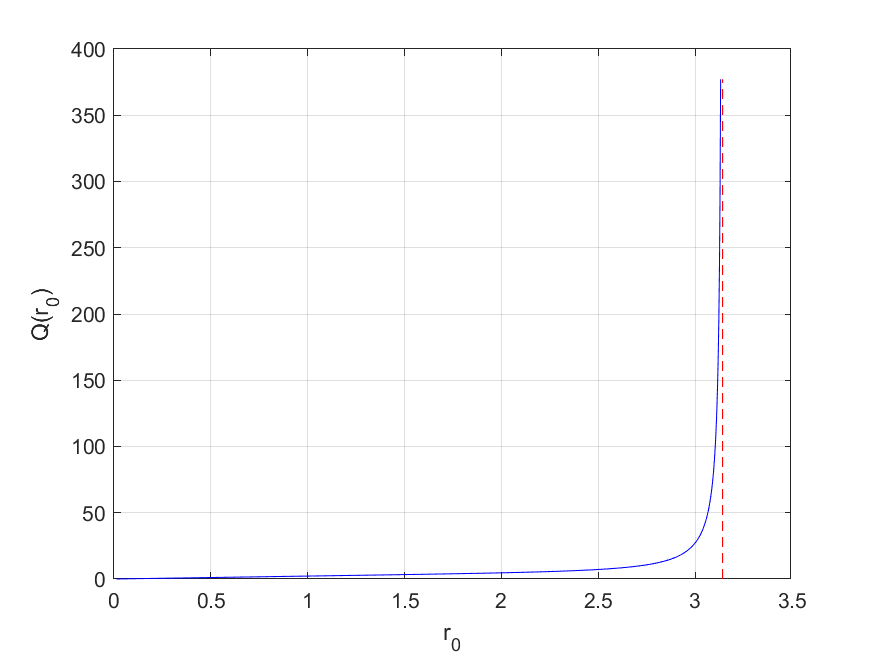
\includegraphics[width=0.8\linewidth]{Qro.png}
    \caption{The plot of \(Q(r_0)\).}
    \label{fig:acrobot-Q}
\end{figure}

Unfortunately there is no \(\delta > 0\) such that \(Q(r_0) \geq \delta\)
everywhere on \(]0,\pi[\), though such a \(\delta\) does exist 
on \(]\omega,\pi[\) for each fixed \(\omega > 0\).
This means all conditions of Lemma \ref{lemma:energy-regulation-D}
are satisfied on the annulus
\[
    D_\omega = \mathcal{O}_1 \backslash 
    \{(q_u,p_u) \in \SxR \mid E(q_u,p_u) \leq E(\omega,0)\}
    .
\]
Therefore, for each \(\omega \in \, ]0,\pi[\) there exists some 
\(I_1(\omega) > 0\) such that the acrobot gains/loses energy everywhere on
\(D_\omega\).
To prove energy gain on all of \(\mathcal{O}_1\), we will show the origin is a
repeller so that all orbits near the origin flow away from the origin into
\(D_\omega\) (for small enough \(\omega\)) and continue gaining energy
thereafter.

Recall the discrete-time pseudo-radius dynamics \eqref{eqn:r-discrete} from the
proof of Lemma \ref{lemma:energy-regulation-D}. 
To prove the origin is a repeller, we need simply
prove the linearization of \eqref{eqn:r-discrete} is greater than \(1\) at 
\(r_0 = 0\). 
This linearization yields
\[
    P^\prime(0) = 1 + I K Q^\prime(0) + R^\prime(2\pi,0,I)
    ,
\]
where the prime now denotes differentiation with respect to \(r\).
One can show that
%\begin{equation*}
%    \lim \limits_{r_0 \to 0^+}
%    \pdiff{a}{r}(\theta,r_0) 
%    = -\frac{\sqrt{2}}{2} \left(11\sin(\theta)^2 - 6\right)
%    ,
%\end{equation*}
%which means
\begin{align*}
    Q^\prime(0) = \int \limits_0^\pi 
    \lim \limits_{r_0 \to 0^+}\pdiff{a}{r}(\sigma,r_0) d\sigma
    = \frac{\pi}{2\sqrt{2}} > 0
    .
\end{align*}
Since \(R(2\pi,0,I)\) is \(O(I^2)\), so is
\(R^\prime(2\pi,0,I)\).
Hence, it can be written in the form
\(I^2 \tilde{R}(I)\) where \(\tilde{R}(I)\) is smooth and zero at \(I = 0\).
Thus, there exists \(I_0 > 0\) such that 
\(I K Q^\prime(0) + I^2 \tilde{R}(I) > 0\) for all \(I \in \, ]0,I_0]\),
which implies \(P^\prime(0) > 1\).
The origin is therefore a repeller, which means there exists some
(unknown) \(\mu > 0\) where \(]0,\mu]\) is negatively
invariant for \eqref{eqn:r-discrete}, and all solutions in this
interval flow through \(r = \mu\).
Hence, all orbits in \(\mathcal{O}_1\) near the
origin will gain energy up to (and including) \(E(\mu,0)\).

Since there exists \(I_1(\mu)\) so that the acrobot gains energy on \(D_\mu\),
taking \(I^\star = \min\{I_0,I_1(\mu)\}\) means the acrobot will gain energy on
\(\mathcal{O}_1\) for each \(I \in \, ]0,I^\star]\).
If \(I < 0\), then \(P^\prime(0) < 1\) and the origin is an
asymptotically stable equilibrium.
Since the acrobot now loses energy on \(D_\mu\), it also loses energy 
on \(\mathcal{O}_1\) for \(I \in [-I^\star,0[\).

We have proved that any acrobot constrained by 
our VNHC \eqref{eqn:acrobot-constraint} gains/loses energy on \(\mathcal{O}_1\).
We must now confirm that the acrobot will begin rotating, 
i.e., that for \(I > 0\) almost every orbit initialized in \(\mathcal{O}_1\)
will reach the line \(|q_u| = \pi\).
Since the definition of energy gain only guarantees that orbits initialized in
\(\mathcal{O}_1\) will escape compact subsets of \(\mathcal{O}_1\) in finite
time, we must first prove that almost every orbit in \(\mathcal{O}_1\) will
escape \(\mathcal{O}_1\) through its boundary, the level set \(E_\pi\) with
energy \(E(\pi,0)\).

Define \(\bar{\mathcal{O}}_1 = \mathcal{O}_1 \cup E_\pi\) to be the closure of
\(\mathcal{O}_1\).
An orbit of the acrobot will only begin rotating if it escapes
\(\bar{\mathcal{O}}_1\) by crossing through \(E_\pi\), and eventually remains
outside this set.
Taking the Jacobian of the constrained dynamics
~\eqref{eqn:acrobot-constrained-dynamics} at the upright equilibrium 
\((q_u,p_u) = (\pi,0)\) yields
\[
    J = \begin{bmatrix}
        -\frac{6mgl\bar{q}_aI}{5} & \frac{1 - 2m^2gl^3\bar{q}_a^2 I^2}{5ml^2} \\
        3mgl & mgl\bar{q}_aI
    \end{bmatrix}
    ,
\]
which has characteristic polynomial
\[
    \det\left(\lambda \Id{2} - J\right)
    = \lambda^2 + \frac{mgl\bar{q}_a I}{5} \lambda - 3g
    .
\]
By Descartes' rule of signs, this polynomial always has exactly one root with
positive real part. 
The equilibrium \((\pi,0)\) is therefore unstable, so the stable manifold
\(\Pi^+\) of initial conditions converging to \((\pi,0)\) is one-dimensional,
and hence is of measure zero in \(\SxR\).

Using \(x(t) := (q_u(t),p_u(t))\) as shorthand, let
\(x(0) \in \mathcal{O}_1\) be a nonzero initial condition of the acrobot.
Suppose by way of contradiction that the orbit \(x(\R)\) is confined within 
\(\bar{\mathcal{O}}_1\), and does not exit through \(E_\pi\) into the rotation
zone.
%Since \(\bar{\mathcal{O}}_1\) is compact, the Birkhoff Theorem \cite{birkhoff}
%implies:
%\begin{itemize}
%    \item The positive limit set \(L_+\) of \(x(t)\) is non-empty, compact, and
%        invariant.
%    \item The solution \(x(t)\) asymptotically tends to \(L_+\).
%\end{itemize}
Since the acrobot gains energy on \(\mathcal{O}_1\) and \(\bar{\mathcal{O}}_1\)
is compact, the Birkhoff Theorem \cite{birkhoff} implies that
the solution \(x(t)\) asymptotically tends to the positive limit set, which is
the largest invariant subset of \(E_\pi\).
Taking the limit as \(r \to \pi\) of
\eqref{eqn:theta-dot-nom-osc}--\eqref{eqn:theta-dot-limit},
we get \(\dot{\theta} \geq 0\) on \(E_\pi\) with equality if and only if
\(\theta \in \{0,\pi\}\).
Thus, the largest invariant subset of \(E_\pi\) is either the upright
equilibrium \(\{(\pi,0)\}\) or \(E_\pi\) itself.

Taking the derivative of \(E(q_u,p_u)\) at the \(p_u\)-axis yields
\(\dot{E}(0,p_u) = g/(5l) \sin(q_a)p_u\).
This is non-zero on \(E_\pi\), so \(E_\pi\) is not invariant and the positive
limit set of \(x(t)\) must be the set \(\{(\pi,0)\}\). 
Hence, \(x(t)\) converges to \((\pi,0)\), so \(x(0) \in \Pi^+\).
Since \(\Pi^+\) is a set of measure zero in \(\SxR\), almost every orbit
initialized in \(\mathcal{O}_1\) must escape at least once through \(E_\pi\)
into the rotation domain.

Using this fact, we now prove that almost every orbit in \(\mathcal{O}_1\) will
cross the line \(|q_u| = \pi\).
Let \(x(0) \in \mathcal{O}_1\) and suppose that the orbit
\(x([0,\infty[)\) does not hit the line \(|q_u| = \pi\).
We claim that this orbit must remain in the compact set 
\(\Sone \times [-K,K]\), for some \(K > 0\).
By contradiction, suppose otherwise.
Then for arbitrary \(K > 0\), there exists some \(t_K > 0\) such that
\(|p_u(t_K)| = K\). 
Looking at the constrained dynamics \eqref{eqn:acrobot-constrained-dynamics},
we see that \(\dot{p}_u \geq -3mgl\) and
\(\dot{q}_u \geq c_1 p_u + c_2\) for some constants \(c_1,c_2 > 0\).
This implies there exists a \(t_{1/2} > 0\) (independent of \(K\)) 
where
\(|p_u(t)| >= K/2\) for \(t \in [t_K, t_K + t_{1/2}]\),
and \(\dot{q}_u \geq c_1 K/2 + c_2\) on this interval.
Picking \(K\) large enough guarantees \(q_u(t)\) covers a distance of \(2\pi\)
over this time interval, and so the orbit must hit the line \(|q_u| = \pi\).
Contradiction.

Thus, the orbit must \(x(t)\) remain within the compact set 
\(\Sone \times [-K,K]\).
By the Birkhoff theorem, \(x(t)\) approaches a positive limit set \(L^+\), 
which is either an invariant closed orbit which crosse the \(q_u\)-axis, 
or the set \(\{(\pi,0)\}\).
By contradiction, suppose \(L^+\) is a closed orbit which 
hits the \(q_u\)-axis at \(\bar{q} < \pi\).
Since \(]0,\mu]\) is negatively invariant for \eqref{eqn:r-discrete}, 
we must have \(\bar{q} \in ]\mu,\pi[\).
The Poincar\'{e} map \eqref{eqn:poincare-map} is smooth on \(]0,\pi[\), and its
image contains \(\bar{q}\), so \(P^{-1}(\bar{q}) \neq \emptyset\).
Take \(q^\prime \in P^{-1}(\bar{q})\). 
If \(q^\prime \in ]0,\mu]\), then \(q^\prime < \bar{q}\).
If \(q^\prime > \mu\), then we know 
from the proof of Lemma \ref{lemma:energy-regulation-D} that
\(P(q^\prime) = \bar{q} \geq q^\prime + \gamma\) for some \(\gamma > 0\), 
so \(q^\prime \leq \bar{q} - \gamma < \bar{q}\).
Since \(q^\prime < \bar{q}\), the orbit starting at \(q^\prime\) stays within
\(\mathcal{O}_1\) and intersects the closed orbit at \(\bar{q}\).
This violates uniqueness of solutions for the constrained dynamics,
so \(L^+\) must be \(\{(\pi,0)\}\), which in turn implies that 
\(x(0) \in \Pi^+\).

We conclude that almost all orbits beginning in \(\mathcal{O}_1\) will
escape the closure of \(\mathcal{O}_1\) and, in finite time, 
begin rotating by crossing the vertical line \(|q_u| = \pi\).

\subsection{Energy Gain on \(\mathcal{O}_2(\rho)\)}
Since \(\mathcal{O}_2(\rho) = \bar{\mathcal{O}}_1 \cup \mathcal{R}(\rho)\)
(where \(\mathcal{R}(\rho)\) is the rotation domain defined in
\eqref{eqn:rotation-domain}), and since all orbits escape 
\(\bar{\mathcal{O}_1}\) in finite time, we need simply prove energy gain on
\(\mathcal{R}(\rho)\) to prove energy gain on \(\mathcal{O}_2(\rho)\).
We separate \(\mathcal{R}(\rho)\) into its two distinct connected components:
\(\mathcal{R}^+(\rho)\), the set of rotations with \(p_u > 0\); 
and \(\mathcal{R}^-(\rho)\), the set of rotations with \(p_u < 0\).
We take the domain of interest for Lemma \ref{lemma:energy-regulation-D} to be
\(D \in \{\mathcal{R}^+(\rho), \mathcal{R}^-(\rho)\}\).

We now apply
\cite[Eqn. (8)]{dynamic_vhcs_stabilize_closed_orbits} to find pseudo-polar coordinates
adapted to rotations.
These coordinates are 
\begin{align}
    \label{eqn:r-rot}
    r &= \sqrt{p_u^2 + 30m^2gl^3(1-c_u)}
    , \\
    \label{eqn:theta-rot}
    \theta &= \alpha(D) q_u
\end{align}
where \((r,\theta) \in \, ]\sqrt{60m^2gl^3}, \rho[ \times \Sone\),
and \(\alpha(D) = 1\) if \(D = \mathcal{R}^+(\rho)\)
or \(-1\) if \(D = \mathcal{R}^-(\rho)\).
The inverse of this transformation is
\begin{align*}
    q_u &= \alpha(D) \theta
    , \\
    p_u &= \alpha(D) \sqrt{r^2-30m^2gl^3(1-c_\theta)}
    .
\end{align*}

In computing the constrained dynamics in
\((r,\theta)\) coordinates and setting \(I = 0\), 
we find that \(\dot{r} \equiv 0\) and
\[
\dot{\theta} = \frac{1}{5ml^2} \sqrt{r^2 - 30m^2gl^3(1-c_\theta)}
,
\]
which is strictly positive as required.
Defining \(g(\theta,r,I) = \dot{r}/\dot{\theta}\), symbolic computations
also confirm that \((\partial g/\partial r)(\theta,r,0) \equiv 0\).
The function \(b(\theta,r_0) = (\partial g/\partial I)(\theta,r_0,0)\) is given
in the statement of Theorem \ref{thm:acrobot-energy-stabilization}, and by
assumption we have \(S(r_0) \geq \epsilon\) on
\(]\sqrt{60m^2gl^3},\rho[\).

All requirements of Lemma \ref{lemma:energy-regulation-D} are satisfied,
so there exists a control parameter \(I_2(\rho) > 0\) whereby the acrobot
gains energy on both \(\mathcal{R}^+(\rho)\) and \(\mathcal{R}^-(\rho)\) for
each \(I \in \, ]0,I_2(\rho)]\).
Let \(I_1^\star\) be the value we found for \(\mathcal{O}_1\) in 
Section \ref{sec:proof-o1}, and let
\(I^{\star\star} = \min \{I_1^\star, I_2(\rho)\}\).
Then the acrobot gains/loses energy on \(\mathcal{O}_2(\rho)\)
for each \(I \in \,]0, I^{\star\star}]\).
If instead \(I \in [-I^{\star\star},0[\), the acrobot dissipates energy on
\(\mathcal{O}_2(\rho)\).

This completes the proof of Theorem \ref{thm:acrobot-energy-stabilization}.

%/========== Conclusion ==========/%
\section{Conclusion}\label{sec:conclusion}

In this article we applied the framework of virtual nonholonomic constraints
to the acrobot, and designed a constraint which emulates giant motion from
gymnastics.
We proved this constraint will inject energy into the simplified acrobot whose
limbs are massless rods of equal length, with equal masses at the tips.
We then performed simulations and physical experiments on a real acrobot robot.
These demonstrated that virtual nonholonomic constraints are capable of
injecting and dissipating energy in a robust manner, while producing
realistic biologically-inspired motion.

%---------- Bibliography ----------%
\bibliography{bib}
\end{document}
%/========== /Main Document ==========/%
% vim: set tw=80 ts=4 sw=4 sts=0 et ffs=unix :
